% Created 2023-04-27 Πεμ 15:25
% Intended LaTeX compiler: pdflatex
\documentclass[11pt]{article}
\usepackage[utf8]{inputenc}
\usepackage[T1]{fontenc}
\usepackage{graphicx}
\usepackage{longtable}
\usepackage{wrapfig}
\usepackage{rotating}
\usepackage[normalem]{ulem}
\usepackage{amsmath}
\usepackage{amssymb}
\usepackage{capt-of}
\usepackage{hyperref}
\usepackage{booktabs}
\usepackage{import}
\usepackage[LGR, T1]{fontenc}
\usepackage[greek, english]{babel}
\usepackage{alphabeta}
\usepackage{esint}
\usepackage{mathtools}
\usepackage{esdiff}
\usepackage{makeidx}
\usepackage{glossaries}
\usepackage{newfloat}
\usepackage{minted}
\usepackage[a4paper, margin=3cm]{geometry}
\usepackage{chemfig}
\usepackage{svg}
\usepackage[a4paper, margin=3cm]{geometry}
\newcommand{\HRule}{\rule{\linewidth}{0.5mm}}
\date{}
\title{Ολοκλήρωση της διεργασίας και κοστολόγηση}
\hypersetup{
 pdfauthor={Vidianos Giannitsis},
 pdftitle={Ολοκλήρωση της διεργασίας και κοστολόγηση},
 pdfkeywords={},
 pdfsubject={},
 pdfcreator={Emacs 28.2 (Org mode 9.5.5)}, 
 pdflang={English}}
\makeatletter
\newcommand{\citeprocitem}[2]{\hyper@linkstart{cite}{citeproc_bib_item_#1}#2\hyper@linkend}
\makeatother

\usepackage[notquote]{hanging}
\begin{document}

\renewcommand{\abstractname}{Περίληψη}
\renewcommand{\tablename}{Πίνακας}
\renewcommand{\figurename}{Σχήμα}
\renewcommand\listingscaption{Κώδικας}

\renewcommand{\contentsname}{Περιεχόμενα}
\begin{titlepage}

\begin{center}
  \begin{minipage}{0.15\textwidth}
    \begin{flushleft}
      \includegraphics[width=1\textwidth]{~/Pictures/ntua_logo.png}\\[0.4cm]    
    \end{flushleft}
  \end{minipage}
  \begin{minipage}{0.80\textwidth}
    \textsc{\bfseries \large ΕΘΝΙΚΟ ΜΕΤΣΟΒΙΟ ΠΟΛΥΤΕΧΝΕΙΟ}\\[0.2cm]
    \textsc{\bfseries \large ΣΧΟΛΗ ΧΗΜΙΚΩΝ ΜΗΧΑΝΙΚΩΝ - ΤΟΜΕΑΣ ΙΙ}\\[0.2cm]
    \textsc{\bfseries \normalsize ΕΡΓΑΣΤΗΡΙΟ ΣΧΕΔΙΑΣΜΟΥ ΚΑΙ ΑΝΑΛΥΣΗΣ ΔΙΕΡΓΑΣΙΩΝ}\\[0.2cm]
  \end{minipage}
  \\[1.5cm]

  \Large Εργασία Μαθήματος <<Σχεδιασμός Διεργασιών>>\\[1.5cm]
  \HRule \\[0.4cm]
  { \textsc{\huge \bfseries Αξιοποίηση Πυρηνόξυλου για Παραγωγή Γλυκερόλης και Κυκλοπεντανόνης - Ολοκλήρωση της Διεργασίας και Κοστολόγηση της}}\\[0.4cm]
  \HRule \\[3cm]

  \begin{minipage}{0.4\textwidth}
    \begin{flushleft} \large
      \emph{Συγγραφείς:}\\
      Βιδιάνος Γιαννίτσης\\
      Αριστοτέλης Αργυρόπουλος\\
      Διονύσης Γιαννάτος\\
      Θεωφανώ Αντωνία Πόταρη\\
      Στυλιανή Σταύρου\\
      Έλλη Πούτα
    \end{flushleft}
  \end{minipage}
  \begin{minipage}{0.4\textwidth}
    \begin{flushright} \large
      \emph{Αριθμοί Μητρώου:}\\
      ch19113\\
      ch19114\\
      ch19074\\
      ch19555\\
      ch19606\\
      ch19534
    \end{flushright}
  \end{minipage}\\[1cm]
  \HRule \\[2cm]

  \vfill
  {\large Αθήνα, 2022}
\end{center}

\end{titlepage}

\tableofcontents
\pagebreak

\section{Υπενθύμιση της διεργασίας}
\label{sec:orgefb165f}
Η διεργασία που έχουμε μελετήσει είναι η αξιοποιήση του πυρηνόξυλου, δηλαδή του ξυλώδους υπολείμματος της επεξεργασίας των αποβλήτων ελαιοτριβείου και η παραγωγή χρήσιμων χημικών όπως η γλυκερόλη και η κυκλοπεντανόνη.

Το πυρηνόξυλο αρχικά πρέπει να κλασματοποιηθεί το οποίο γίνεται με έκρηξη ατμού και έπειτα αλκαλική εκχύλιση και bleaching της λιγνίνης. Το κυτταρινικό κλάσμα υδρολύεται προς γλυκόζη και έπειτα χρησιμοποιείται σε μία καθαρή καλλιέργεια του μικροοργανισμού Candida glycerinogenes για παραγωγή γλυκερόλης η οποία ανακτάται με ένα flash (για απομάκρυνση του νερού) και έπειτα μία απόσταξη (για περαιτέρω καθαρισμό της γλυκερόλης).

Το ημικυτταρινικό κλάσμα αυτουδρολύεται κατά την έκρηξη ατμού από τις έντονες συνθήκες και πηγαίνει για παραγωγή κυκλοπεντανόνης. Ως πλατφόρμα για την παραγωγή αυτή, χρησιμοποιείται η φουρφουράλη, ένα προιόν αφυδάτωσης της ξυλόζης σε υψηλή θερμοκρασία. Η καταλυτική υδρογόνωση της φουρφουράλης σε υψηλή πίεση παράγει την επιθυμητή κυκλοπεντανόνη. Βέβαια, το μίγμα νερό-κυκλοπεντανόνη είναι ένα δύσκολο μίγμα στον διαχωρισμό λόγω της δημιουργίας αζεοτρόπου, συν ότι υπάρχει και περίσσεια φουρφουράλης στον αντιδραστήρα η οποία δημιουργεί και αυτή αζεότροπο. Αν η απόσταξη γίνει σε υψηλή πίεση (πχ στα 40 bar που είναι ήδη το ρεύμα) δεν υπάρχει το πρόβλημα αυτό, όμως η απόσταξη είναι πολύ δύσκολη, λόγω της υψηλής πίεσης και τίθενται και θέματα ασφάλειας. Για αυτό, προτείνεται η ψύξη του ρεύματος μέχρι θερμοκρασία περιβάλλοντος (μαζί με εκτόνωση σε ατμοσφαιρική πίεση), εκχύλιση της κυκλοπεντανόνης από το νερό με τολουόλιο και έπειτα απόσταξη του μίγματος η οποία είναι αρκετά εύκολη καθώς το τολουόλιο είναι αρκετά πτητικό.

Τέλος, η λιγνίνη της διεργασίας καίγεται και χρησιμοποιείται σε κύκλο συμπαραγωγής θερμικής και ηλεκτρικής ενέργειας.

Καθώς η διεργασία αυτή είναι πολύ μεγάλη, παρακάτω έχει ακολουθηθεί μία θεώρηση με blocks τα οποία χωρίζουν σε κομμάτια την διεργασία ώστε να είναι πιο κατανοητή.

\section{Αναγνώριση των blocks και των ρευμάτων σε αυτά}
\label{sec:org258461e}
Για την καλύτερη κατανόηση της διεργασίας, θα αναλυθεί ξεχωριστά κάθε block, οι διεργασίες σε αυτό και τα θερμά και ψυχρά του ρεύματα. Αξίζει να αναφερθεί πως οι φωτογραφίες του κάθε block στο Aspen οι οποίες παρατίθενται είναι πριν την συνολική ενεργειακή ολοκλήρωση της μονάδας και άρα οι περισσότερες εκ αυτών δεν είναι πλέον έγκυρες. Οι τελικές μορφές τους θα αναφερθούν κατά τον σχεδιασμό του τελικού δικτύου εναλλαγής θερμότητας.

\subsection{Block 100 - Κλασμάτωση της βιομάζας}
\label{sec:org10ba554}
Το block αυτό είναι για την βασική διεργασία διαχωρισμού την έκρηξη ατμού και της επακόλουθες διεργασίες διαχωρισμού κυτταρίνης-λιγνίνης. Ως τροφοδοσία έχει νερό για παραγωγή ατμού, πυρηνόξυλο (πρώτη ύλη) και τα υδατικά διαλύματα που απαιτούνται για τις διεργασίες διαχωρισμού. Προιόντα είναι τα τρία βασικά ρεύματα ξυλόζης, κυτταρίνης και λιγνίνης.

\begin{figure}[htbp]
\centering
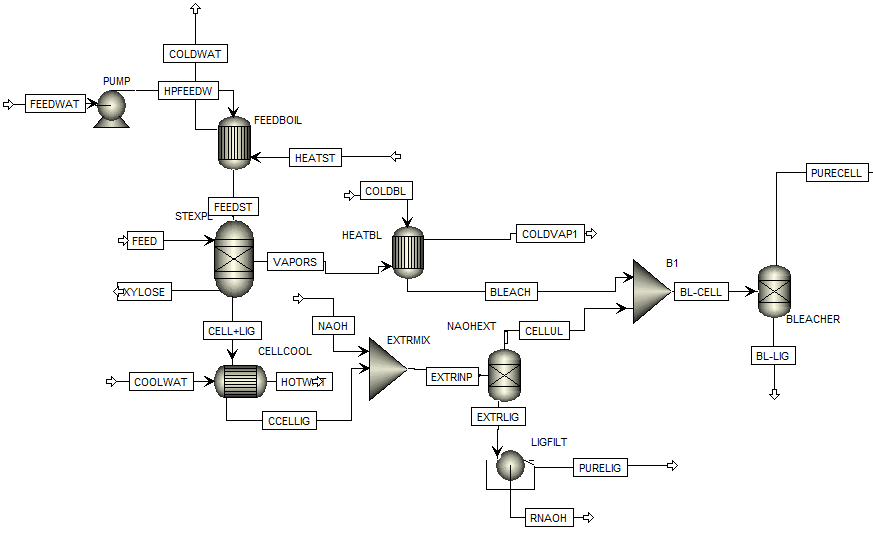
\includegraphics[width=.9\linewidth]{Block_100_-_Διαχωρισμός_των_τριών_κομματιών_της_βιομάζας/2023-03-11_15-21-38_screenshot.png}
\caption{Block 100 στο Aspen}
\end{figure}

Στο block αυτό, έχουμε τα εξής.
\begin{itemize}
\item Aτμός της τροφοδοσίας ο οποίος θερμαίνεται από θερμοκρασία περιβάλλοντος μέχρι 232 \(^oC\) (ψυχρό ρεύμα). Το ρεύμα με το οποίο εναλλάσσει θερμότητα είναι βοηθητική παροχή της διεργασίας. Κάποια από την θερμότητα του προσφέρεται για την θέρμανση και διάσπαση του πυρηνόξυλου, ενώ ο υπόλοιπος ατμός, μαζί με τα υπόλοιπα ατμώδη υπολείμματα της έκρηξης (κυρίως CO\textsubscript{2}) διατίθενται ως ένα θερμό ρεύμα της διεργασίας. Βέβαια, αν παρατηρηθεί πως υπάρχει περίσσεια θερμικής ενέργειας, μπορεί αυτό το ρεύμα να μην χρησιμοποιηθεί.
\item Κυτταρίνη και Λιγνίνη που βγαίνουν από το steam explosion στους 232 και πρέπει να ψυχθούν μέχρι την θερμοκρασία λειτουργίας της αλκαλικής εκχύλισης (80 \(^oC\)). Μπορούμε να εκμεταλλευτούμε το υπάρχον θερμικό περιεχόμενο τους για να θερμάνουμε και το διάλυμα καυστικού νατρίου όμως. Η θερμοκρασία βγαίνει 80.65 \(^oC\) αν ο εναλλάκτης το ψύξει μέχρι τους 105 \(^oC\).
\item Η ξυλόζη οδηγείται στην διεργασία παραγωγής κυκλοπεντανόνης, για αυτό για το block αυτό δεν μεταβάλλεται η θερμότητα της.
\item Θέρμανση του διαλύματος χλωρίνης (bleach) καθώς για την πλήρη απολιγνοποίση θέλουμε εφαρμογή του διαλύματος αυτού στους 70 \(^oC\) (ψυχρό ρεύμα). Στο παρόν διάγραμμα ροής γίνεται εν μέρει με την θερμότητα των ατμών της έκρηξης ατμού και μετά με την ανάμιξη με το ρεύμα κυτταρίνης για τελική θερμοκρασία 69.9 \(^oC\). Στην ανάμιξη αυτή έχουμε και μείωση της θερμότητας του ρεύματος κυτταρίνης κατά 10 \(^oC\) περίπου.

Άρα μπορούμε να κάνουμε τον εξής πίνακα για τα εκμεταλλεύσιμα θερμά και ψυχρά ρεύματα
\end{itemize}

\begin{longtable}{llrrrl}
\caption{Θερμά και Ψυχρά Ρεύματα στο Block 100}
\\
Ρεύμα & Είδος & Τ\textsubscript{in} (C) & Τ\textsubscript{out} (C) & Παροχή (kmol/hr) & Σύσταση\\
\hline
\endfirsthead
\multicolumn{6}{l}{Continued from previous page} \\
\hline

Ρεύμα & Είδος & Τ\textsubscript{in} (C) & Τ\textsubscript{out} (C) & Παροχή (kmol/hr) & Σύσταση \\

\hline
\endhead
\hline\multicolumn{6}{r}{Continued on next page} \\
\endfoot
\endlastfoot
\hline
FeedSteam & Ψυχρό & 20 & 232 & 633.22 & Νερό\\
\hline
Vapors & Θερμό & 232 & 30 & 905.27 & Νερό 0.92\\
 &  &  &  &  & CO\textsubscript{2} 0.08\\
\hline
CellLig & Θερμό & 232 & 80.65 & 84.76 & Κυτταρίνη 0.5\\
 &  &  &  &  & Λιγνίνη 0.5\\
\hline
NaOH & Ψυχρό & 20 & 80.65 & 80.37 & Νερό\\
\hline
Bleach & Ψυχρό & 20 & 69.9 & 55.62 & Νερό 99.5\\
 &  &  &  &  & Χλωρίνη 0.05\\
\hline
Cellulose & Θέρμο & 80.65 & 69.9 & 54.32 & Κυτταρίνη 0.78\\
 &  &  &  &  & Λιγνίνη 0.22\\
\hline
\end{longtable}

\subsection{Block 200 - Παραγωγή Γλυκόζης}
\label{sec:orgd41281d}
Σκοπός του block αυτού είναι η υδρόλυση της κυτταρίνης και παραγωγή καθαρής γλυκόζης που μπορεί να χρησιμοποιηθεί ως θρεπτικό μέσο στην καλλιέργεια του C. glycerinogenes. Στο block αυτό θεωρείται ως τροφοδοσία η καθαρή κυτταρίνη του block 100 και νερό το οποίο απαιτείται για την υδρόλυση της κυτταρίνης. Προιόν της διεργασίας είναι η γλυκόζη που θα τροφοδοτηθεί στον βιοαντιδραστήρα παραγωγής γλυκερόλης (block 400).

\begin{figure}[htbp]
\centering
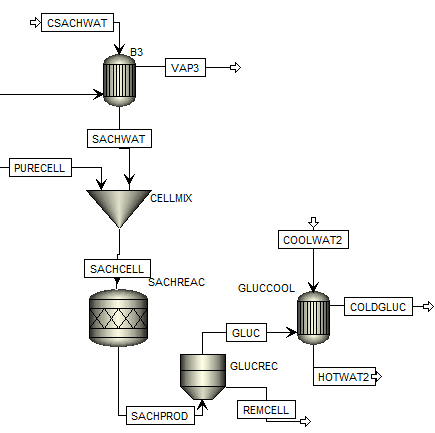
\includegraphics[width=300px]{Block_200_-_Παραγωγή_Γλυκόζης/2023-03-11_16-51-41_screenshot.png}
\caption{Block 200 στο Aspen}
\end{figure}


Στο block αυτό:
\begin{itemize}
\item Θέλουμε η κυτταρίνη και το νερό να τροφοδοτηθούν στους 50 \(^oC\) για την υδρόλυση. Για αυτό, το νερό πρώτα θερμαίνεται μέχρι μία θερμόκρασία και μετά αναμιγνύεται με την κυτταρίνη για τελική θερμοκρασία 49.75 \(^oC\). Το νερό ξεκινάει από θερμοκρασία περιβάλλοντος και θερμαίνεται (επειδή η θερμοκρασία θα πέσει πολύ αν αναμιχθούν ως έχει) ενώ η κυτταρίνη ψύχεται από τους 69.9 \(^oC\).
\item Η γλυκόζη ψύχεται από τους 50 \(^oC\) στους οποίους παράχθηκε μέχρι τους 30 \(^oC\) η οποία είναι η βέλτιστη λειτουργία του αντιδραστήρα παραγωγής γλυκερόλης στο block 400.

Άρα μπορούμε να κάνουμε τον εξής πίνακα για τα εκμεταλλεύσιμα θερμά και ψυχρά ρεύματα
\end{itemize}
\begin{table}[htbp]
\caption{Θερμά και Ψυχρά Ρεύματα στο Block 200}
\centering
\begin{tabular}{llrrrl}
Ρεύμα & Είδος & Τ\textsubscript{in} (C) & Τ\textsubscript{out} (C) & Παροχή (kmol/hr) & Σύσταση\\
\hline
PureCell & Θερμό & 61.97 & 49.75 & 42.55 & Κυτταρίνη\\
\hline
SachWater & Ψυχρό & 20 & 49.75 & 715 & Νερό\\
\hline
Glucose & Θερμό & 50 & 30 & 669.45 & Νερό 0.97\\
 &  &  &  &  & Γλυκόζη 0.03\\
\hline
\end{tabular}
\end{table}

\subsection{Block 300 - Λέβητας Καύσης Λιγνίνης}
\label{sec:org2c1deb2}
To block αυτό έχει την προσομοίωση του λέβητα που χρησιμοποιείται για την καύση της λιγνίνης και του κύκλου συμπαραγωγής θερμικής και ηλεκτρικής ενέργειας. Η λιγνίνη καίγεται και από τα καυσαέρια της παράγεται ατμός υψηλής πίεσης. Προιόν του block 300 είναι ο ατμός υψηλής πίεσης που είναι αρκετά χρήσιμος για την εγκατάσταση. Αν χρησιμοποιηθεί όλη η λιγνίνη για παραγωγή ατμού ο οποίος θα διατεθεί ως θερμαντικό μέσο, μιλάμε για ένα θερμό ρεύμα με ενθαλπία 88.6 MW. Παρότι δεν έχουν αναφερθεί ακόμη οι ενεργειακές απαιτήσεις των διεργασιών, μία πρόχειρη προσέγγιση μας λέει πως όλες οι διεργασίες που έχουμε, χωρίς καμία ολοκλήρωση έχουν απαίτηση σε θερμή βοηθητική παροχή 23 MW. Άρα υπάρχει μία μεγάλη περίσσεια θερμικής ενέργειας, η οποία όταν υπάρχει σε μία εγκατάσταση χρησιμοποιείται για ηλεκτροπαραγωγή.

\begin{figure}[htbp]
\centering
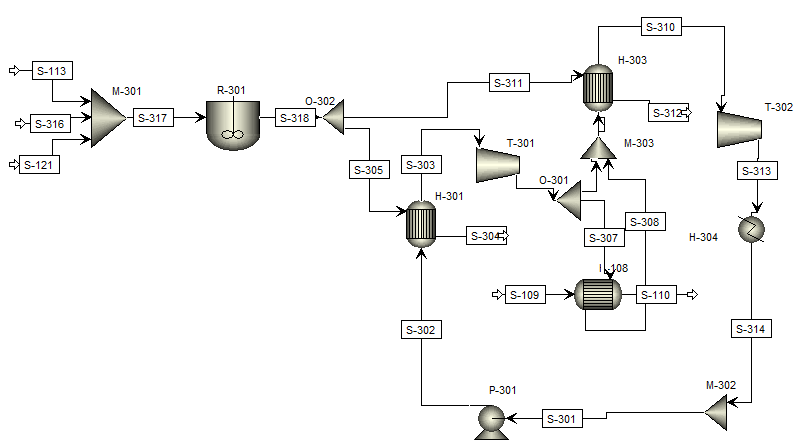
\includegraphics[width=.9\linewidth]{Αναγνώριση_των_blocks_και_των_ρευμάτων_σε_αυτά/2023-04-27_13-13-25_screenshot.png}
\caption{Block 300 στο Aspen}
\end{figure}


Εφόσον αυτό το block χρησιμοποιεί ένα κύκλο Rankine για ηλεκτροπαραγωγή (λόγω της τεράστιας περίσσειας θερμικής ενέργειας που έχει), τα ρεύματα του δεν θα ληφθούν υπόψην στην ολοκλήρωση της διεργασίας, αλλά όπου χρειάζεται βοηθητική θερμή παροχή θα υποθέτεται ότι είναι η παροχή S-307 του διαγράμματος αυτού, η οποία είναι ατμός στα 60 bar και 497.5 \(^oC\) και η ποσότητα της θα είναι τέτοια ώστε να είναι αρκετή για όλα τα θερμά της διεργασίας.

\subsection{Block 400 - Παραγωγή Γλυκερόλης}
\label{sec:org6390c85}
Στο block αυτό φαίνεται ο βιοαντιδραστήρας του μικροοργανισμού C. glycerinogenes ο οποίος χρησιμοποιείται για την παραγωγή γλυκερόλης. Ως τροφοδοσία χρησιμοποιείται ένα μίγμα υδατικού διαλύματος γλυκόζης μαζί με ουρία (πηγή αζώτου) και επαρκές οξυγόνο για την αερόβια καλλιέργεια. Επίσης στο feed υπάρχει και μικρή ποσότητα βιομάζας για να ξεκινήσει η αντίδραση.

\begin{figure}[htbp]
\centering
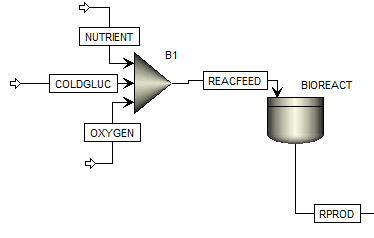
\includegraphics[width=.9\linewidth]{2023-03-11_17-15-10_screenshot.png}
\caption{Block 400 στο Aspen}
\end{figure}

Στο block αυτό, όλα τα ρεύματα τροφοδοτούνται στους 30 \(^oC\) και αντιδρούν σε αντιδραστήρα σταθερής θερμοκρασίας. Άρα, δεν υπάρχει καμία μεταβολή στην θερμοκρασία των ρευμάτων και άρα κανένα θερμό ή ψυχρό ρεύμα να χρησιμοποιηθεί.

\subsection{Block 500 - Καθαρισμός Γλυκερόλης}
\label{sec:org34a4c52}
Το block αυτό είναι για τον διαχωρισμό των προιόντων του βιοαντιδραστήρα και την ανάκτηση της καθαρής εμπορεύσιμης γλυκερόλης. Τροφοδοσία του είναι το προιόν του block 400, δηλαδή τα προιόντα του βιοαντιδραστήρα μετά την πρώτη βαθμίδα θέρμανσης από την γλυκερόλη. Προιόν της διεργασίας είναι η καθαρή γλυκερόλη και δύο υδατικά κλάσματα τα οποία χρησιμοποιούνται για την θέρμανση.

\begin{figure}[htbp]
\centering
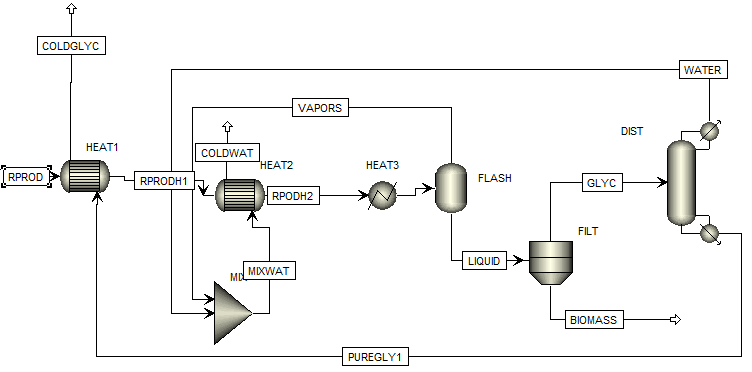
\includegraphics[width=.9\linewidth]{2023-03-11_17-17-18_screenshot.png}
\caption{Block 500 στο Aspen}
\end{figure}

Στο block αυτό υπάρχουν:
\begin{itemize}
\item Θέρμανση του προιόντος του βιοαντιδραστήρα μέχρι τους 140 \(^oC\) για flash και έπειτα απόσταξη (ψυχρό ρεύμα).
\item Παραγωγή 3 διαθέσιμων θερμών ρευμάτων, ένα την ατμώδη φάση του flash, ένα με σχεδόν καθαρό νερό από το απόσταγμα της αποστακτικής και ένα καθαρής γλυκερόλης.

Ο χαρακτηρισμός των ρευμάτων αυτών είναι
\end{itemize}
\begin{center}
\begin{tabular}{llrrrl}
Ρεύμα & Είδος & Τ\textsubscript{in} (C) & Τ\textsubscript{out} (C) & Παροχή (kmol/hr) & Σύσταση\\
\hline
RProd & Ψυχρό & 30 & 140 & 774.29 & Νερό 0.89\\
 &  &  &  &  & CO\textsubscript{2} 0.08\\
 &  &  &  &  & Γλυκερόλη 0.02\\
 &  &  &  &  & Άλλα 0.01\\
\hline
FlashVaps & Θερμό & 140 & 30 & 745.99 & Νερό 0.91\\
 &  &  &  &  & CO\textsubscript{2} 0.089\\
 &  &  &  &  & Άλλα 0.01\\
\hline
GlycWater & Θερμό & 144.4 & 30 & 9.82 & Νερό\\
\hline
PureGlycerol & Θερμό & 288.9 & 30 & 15.9 & Γλυκερόλη\\
\hline
\end{tabular}
\end{center}

Αξίζει να αναφερθεί πως ο χαρακτηρισμός άλλα αναφέρεται σε περίσσεια αντιδρώντων (ουρία, οξυγόνο), την παραγόμενη βιομάζα και τα παραπροιόντα της αντίδρασης (οξικό οξύ και αιθανόλη) τα οποία είναι σε αρκετά μικρές ποσότητες συγκριτικά με το νερό, το CO\textsubscript{2} και την γλυκερόλη. Στους υπολογισμούς της ενεργειακής ολοκλήρωσης θα αγνοηθούν.

\subsection{Block 600 - Παραγωγή Κυκλοπεντανόνης με την Φουρφουράλη ως Ενδιάμεσο}
\label{sec:org266bfcc}
Το block αυτό είναι αυτό που αξιοποιεί την ημικυτταρινική φάση της βιομάζας όπως αυτή βγαίνει από το steam explosion στο block 100. Στο block αυτό παράγεται αρχικά ένα ενδιάμεσο προιόν, η φουρφουράλη, από την αφυδάτωση της ξυλόζης ενώ αυτή οδηγείται σε έναν δεύτερο αντιδραστήρα, όπου με διεργασία καταλυτικής υδρογόνοσης, η φουρφουράλη μετατρέπεται σε κυκλοπεντανόνη, το τελικό μας προιόν.

\begin{figure}[htbp]
\centering
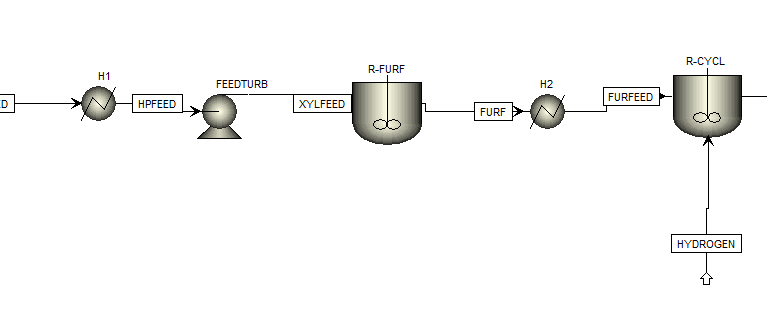
\includegraphics[width=.9\linewidth]{Block_600_-_Παραγωγή_Κυκλοπεντανόνης_με_την_Φουρφουράλη_ως_Ενδιάμεσο/2023-03-11_17-58-53_screenshot.png}
\caption{Block 600 στο Aspen}
\end{figure}

Στο block αυτό:
\begin{itemize}
\item Τροφοδοτείται αρχικά η ξυλόζη στους 232 \(^oC\) όπως βγήκε από την έκρηξη ατμού και θερμαίνεται μέχρι τους 243 \(^oC\) όπου λειτουργεί ο πρώτος αντιδραστήρας (ψυχρό ρεύμα)
\item Ψύχεται το προιόν της πρώτης αντίδρασης για να τροφοδοτηθεί στους 160 \(^oC\) στον 2ο αντιδραστήρα (θερμό ρεύμα).

Άρα τα διαθέσιμα ρεύματα είναι
\end{itemize}
\begin{table}[htbp]
\caption{Θερμά και Ψυχρά Ρεύματα στο Block 600}
\centering
\begin{tabular}{llrrrl}
Ρεύμα & Είδος & Τ\textsubscript{in} (C) & Τ\textsubscript{out} (C) & Παροχή (kmol/hr) & Σύσταση\\
\hline
XylFeed & Ψυχρό & 232 & 243 & 26.38 & Ξυλόζη\\
\hline
FurFeed & Θερμό & 243 & 160 & 105.52 & Νερό 0.75\\
 &  &  &  &  & Φουρφουράλη 0.25\\
\hline
\end{tabular}
\end{table}

\subsection{Block 700 - Καθαρισμός της Κυκλοπεντανόνης}
\label{sec:org66f2e0b}
Το block αυτό έχει ως σκοπό τον καθαρισμό του προιόντος του block 600, δηλαδή του προιόντος του αντιδραστήρα της κυκλοπεντανόνης. Αυτό είναι μίγμα νερού-κυκλοπεντανόνης με μικρή περίσσεια φουρφουράλης και υδρογόνου από την αντίδραση. Προιόν της διεργασίας αυτής είναι η εμπορεύσιμη πλέον κυκλοπεντανόνη υψηλής καθαρότητας. Όπως προαναφέρθηκε, αυτό είναι δύσκολο να γίνει με απόσταξη λόγω αζεοτρόπων για αυτό γίνεται με εκχύλιση.

\begin{figure}[htbp]
\centering
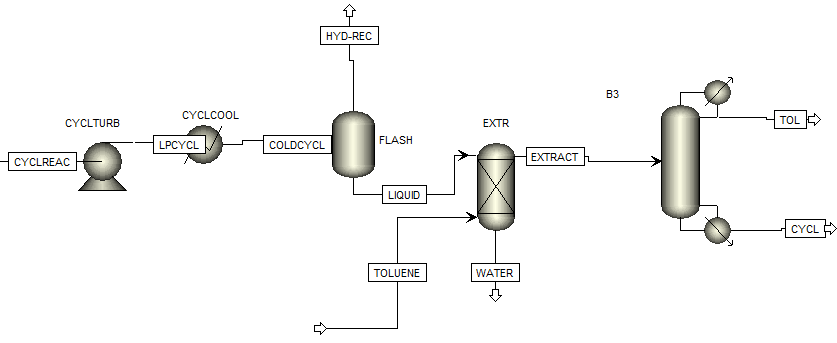
\includegraphics[width=.9\linewidth]{Block_700_-_Καθαρισμός_της_Κυκλοπεντανόνης/2023-03-17_18-13-36_screenshot.png}
\caption{Block 700 στο Aspen}
\end{figure}

Αρχικά το προιόν έρχεται σε θερμοκρασία και πίεση περιβάλλοντος. Έπειτα, περνάει ένα flash για να φύγει το αέριο υδρογόνο, μία εκχύλιση για να φύγει το νερό και τέλος μία απόσταξη για να διαχωριστεί η κυκλοπεντανόνη από τον διαλύτη (τολουόλιο). Το υδρογόνο και το νερό που απομακρύνονται είναι σε θερμοκρασία περιβάλλοντος άρα η θερμική τους εκμετάλλευση δεν έχει ιδιαίτερο νόημα.

\begin{table}[htbp]
\caption{Θερμά και Ψυχρά Ρεύματα στο Block 700}
\centering
\begin{tabular}{llrrrl}
Ρεύμα & Είδος & Τ\textsubscript{in} (C) & Τ\textsubscript{out} (C) & Παροχή (kmol/hr) & Σύσταση\\
\hline
CyclReac & Θερμό & 160 & 30 & 2132.66 & Κυκλοπεντανόνη 0.2\\
 &  &  &  &  & Νερό 0.79\\
 &  &  &  &  & Υδρογόνο 0.01\\
\hline
Cycl & Θερμό & 130 & 30 & 26 & Κυκλοπεντανόνη 0.98\\
 &  &  &  &  & Φουρφουράλη 0.015\\
 &  &  &  &  & Τολουόλιο 0.005\\
\hline
Tol & Θερμό & 50 & 30 & 51.02 & Τολουόλιο 0.98\\
 &  &  &  &  & Νερό 0.01\\
 &  &  &  &  & Κυκλοπεντανόνη 0.01\\
\hline
\end{tabular}
\end{table}

\section{Συνολική εικόνα των ρευμάτων}
\label{sec:orgf4184bd}
Έχοντας δει κάθε block της διεργασίας ξεχωριστά, μπορούμε πλέον να φτιάξουμε τον συνολικό πίνακα θερμών και ψυχρών ρευμάτων ο οποίος είναι και αυτός που θα χρησιμοποιηθεί για την ενεργειακή ολοκλήρωση παρακάτω.

\begin{longtable}{llrrrl}
\caption{Συνολικός Πίνακας Θερμών και Ψυχρών της διεργασίας}
\\
\hline
Ρεύμα & Είδος & Τ\textsubscript{in} (C) & Τ\textsubscript{out} (C) & Παροχή (kmol/hr) & Σύσταση\\
\hline
\endfirsthead
\multicolumn{6}{l}{Continued from previous page} \\
\hline

Ρεύμα & Είδος & Τ\textsubscript{in} (C) & Τ\textsubscript{out} (C) & Παροχή (kmol/hr) & Σύσταση \\

\hline
\endhead
\hline\multicolumn{6}{r}{Continued on next page} \\
\endfoot
\endlastfoot
\hline
FeedSteam & Ψυχρό & 20 & 232 & 633.22 & Νερό\\
\hline
Vapors & Θερμό & 232 & 30 & 905.27 & Νερό 0.92\\
 &  &  &  &  & CO\textsubscript{2} 0.08\\
\hline
CellLig & Θερμό & 232 & 80.65 & 84.76 & Κυτταρίνη 0.5\\
 &  &  &  &  & Λιγνίνη 0.5\\
\hline
NaOH & Ψυχρό & 20 & 80.65 & 80.37 & Νερό\\
\hline
Bleach & Ψυχρό & 20 & 69.9 & 55.62 & Νερό 99.5\\
 &  &  &  &  & Χλωρίνη 0.05\\
\hline
Cellulose & Θέρμο & 80.65 & 69.9 & 54.32 & Κυτταρίνη 0.78\\
 &  &  &  &  & Λιγνίνη 0.22\\
\hline
PureCell & Θερμό & 61.97 & 49.75 & 42.55 & Κυτταρίνη\\
\hline
SachWater & Ψυχρό & 20 & 49.75 & 715 & Νερό\\
\hline
Glucose & Θερμό & 50 & 30 & 669.45 & Νερό 0.97\\
 &  &  &  &  & Γλυκόζη 0.03\\
\hline
RProd & Ψυχρό & 30 & 140 & 774.29 & Νερό 0.89\\
 &  &  &  &  & CO\textsubscript{2} 0.08\\
 &  &  &  &  & Γλυκερόλη 0.02\\
 &  &  &  &  & Άλλα 0.01\\
\hline
FlashVaps & Θερμό & 140 & 30 & 745.99 & Νερό 0.91\\
 &  &  &  &  & CO\textsubscript{2} 0.089\\
 &  &  &  &  & Άλλα 0.01\\
\hline
GlycWater & Θερμό & 144.4 & 30 & 9.82 & Νερό\\
\hline
PureGlycerol & Θερμό & 288.9 & 30 & 15.9 & Γλυκερόλη\\
\hline
XylFeed & Ψυχρό & 232 & 243 & 26.38 & Ξυλόζη\\
\hline
FurFeed & Θερμό & 243 & 160 & 105.52 & Νερό 0.75\\
 &  &  &  &  & Φουρφουράλη 0.25\\
\hline
CyclReac & Θερμό & 160 & 30 & 2132.66 & Κυκλοπεντανόνη 0.2\\
 &  &  &  &  & Νερό 0.79\\
 &  &  &  &  & Υδρογόνο 0.01\\
\hline
Cycl & Θερμό & 130 & 30 & 26 & Κυκλοπεντανόνη 0.98\\
 &  &  &  &  & Φουρφουράλη 0.015\\
 &  &  &  &  & Τολουόλιο 0.005\\
\hline
Tol & Θερμό & 50 & 30 & 51.02 & Τολουόλιο 0.98\\
 &  &  &  &  & Νερό 0.01\\
 &  &  &  &  & Κυκλοπεντανόνη 0.01\\
\hline
\end{longtable}

Για να προετοιμάσουμε τα ρεύματα για την ολοκλήρωση όμως πρέπει αρχικά να υπολογιστεί η θερμοχωρητικότητα του κάθε ρεύματος, διαδικασία που φαίνεται παρακάτω.

\begin{table}[htbp]
\caption{Θερμοχωρητικότητες ουσιών}
\centering
\begin{tabular}{lr}
Ουσία & Cp (J/mol K)\\
\hline
Νερό & 75.38\\
Κυτταρίνη & 89.63\\
Λιγνίνη & 90.98\\
Γλυκόζη & 225\\
Γλυκερόλη & 225.4\\
CO\textsubscript{2} & 37.35\\
Ξυλόζη & 178.1\\
Φουρφουράλη & 159.5\\
Κυκλοπεντανόνη & 112.18\\
Υδρογόνο & 14.5\\
Τολουόλιο & 158.4\\
\hline
\end{tabular}
\end{table}

και από αυτά υπολογίζονται οι ειδικές θερμοχωρητικότητες και οι θερμοχωρητικότητες των ρευμάτων
\begin{longtable}{lrrr}
\caption{Θερμοχωρητικότητες ρευμάτων}
\\
Ρεύμα & Παροχή (kmol/h) & Cp (J/mol K) & CP (MJ/h K)\\
\hline
\endfirsthead
\multicolumn{4}{l}{Continued from previous page} \\
\hline

Ρεύμα & Παροχή (kmol/h) & Cp (J/mol K) & CP (MJ/h K) \\

\hline
\endhead
\hline\multicolumn{4}{r}{Continued on next page} \\
\endfoot
\endlastfoot
\hline
FeedSteam & 633.22 & 75.38 & 47.732124\\
StExpVapors & 905.27 & 72.34 & 65.487232\\
CellLig & 84.76 & 90.31 & 7.6546756\\
NaOH & 80.37 & 75.38 & 6.0582906\\
Bleach & 55.62 & 75.38 & 4.1926356\\
Cellulose & 54.32 & 89.93 & 4.8849976\\
PureCell & 42.55 & 89.63 & 3.8137565\\
SachWater & 715 & 75.38 & 53.8967\\
Glucose & 669.45 & 79.87 & 53.468972\\
RProd & 774.29 & 74.58 & 57.746548\\
FlashVapors & 745.99 & 71.96 & 53.681440\\
GlycWater & 9.82 & 75.38 & 0.7402316\\
PureGlyc & 15.9 & 225.4 & 3.58386\\
XylFeed & 26.38 & 178.1 & 4.698278\\
FurFeed & 105.52 & 96.41 & 10.173183\\
CyclReac & 24.61 & 112.71 & 2.7737931\\
CyclWater & 106.9 & 76.12 & 8.137228\\
\end{longtable}

Επίσης χρήσιμος για την ενεργειακή ολοκλήρωση είναι ο πίνακας των ανηγμένων θερμοκρασιών:

\begin{table}[htbp]
\caption{Πίνακας ανηγμένων θερμοκρασιών}
\centering
\begin{tabular}{llrr}
Ρεύμα & Είδος & Τ\textsubscript{in} (C) & T\textsubscript{out} (C)\\
\hline
FeedSteam & Ψυχρό & 25 & 237\\
StExpVapors & Θερμό & 227 & 25\\
CellLig & Θερμό & 227 & 75.65\\
NaOH & Ψυχρό & 25 & 85.65\\
Bleach & Ψυχρό & 25 & 74.9\\
Cellulose & Θερμό & 75.65 & 64.9\\
PureCell & Θερμό & 56.97 & 44.75\\
SachWater & Ψυχρό & 25 & 54.75\\
Glucose & Θερμό & 45 & 25\\
RProd & Ψυχρό & 35 & 145\\
FlashVaps & Θερμό & 135 & 25\\
GlycWater & Θερμό & 139.4 & 25\\
PureGlycerol & Θερμό & 283.9 & 25\\
XylFeed & Ψυχρό & 237 & 248\\
FurFeed & Θερμό & 238 & 155\\
Cyclo & Θερμό & 262.8 & 25\\
CyclWater & Θερμό & 196.5 & 25\\
\end{tabular}
\end{table}

\section{Ενεργειακή ολοκλήρωση μονάδας}
\label{sec:orgd7f7a80}
Με βάση τους δύο παραπάνω πίνακες, μπορεί να γίνει η συνολική ενεργειακή ολοκλήρωση της μονάδας. Πρώτο βήμα είναι να αναγνωρίσουμε τα θερμά και ψυχρά ρεύματα της διεργασίας, το οποίο έγινε ενώ το δεύτερο είναι να προχωρήσουμε από θερμά και ψυχρά ρεύματα στον ενεργειακό καταρράκτη της διεργασίας και στα συνδυασμένα "ψεύδο"-ρεύματα για κάθε θερμοκρασιακή περιοχή του. Αυτά φαίνονται παρακάτω.

\begin{figure}[htbp]
\centering
\includesvg[width=.9\linewidth]{./Diagrams/energy_cascade}
\caption{Ενεργειακός καταρράκτης της διεργασίας}
\end{figure}

\begin{table}[htbp]
\caption{Χαρακτηρισμός των "ψευδο"-ρευμάτων του ενεργειακού καταρράκτη}
\centering
\begin{tabular}{rrrrrrr}
Τ\textsubscript{1} & T\textsubscript{2} & ΔΤ & CPc & CPh & CP & ΔΗ\\
\hline
283.9 & 248 & 35.9 & 0 & 3.584 & -3.584 & -128.6656\\
248 & 238 & 10 & 4.698 & 3.584 & 1.114 & 11.14\\
238 & 237 & 1 & 4.698 & 13.757 & -9.059 & -9.059\\
237 & 230.01 & 6.99 & 47.732 & 13.757 & 33.975 & 237.48525\\
230 & 227 & 3 & 47.732 & 13.757 & 33.975 & 101.925\\
227 & 155 & 72 & 47.732 & 83.315 & -35.583 & -2561.976\\
155 & 145 & 10 & 47.732 & 91.792 & -44.06 & -440.6\\
145 & 139.4 & 5.6 & 105.479 & 91.792 & 13.687 & 76.6472\\
139.4 & 135 & 4.4 & 105.479 & 92.532 & 12.947 & 56.9668\\
135 & 125 & 10 & 105.479 & 161.279 & -55.8 & -558.\\
125 & 97.01 & 27.99 & 105.479 & 150.889 & -45.41 & -1271.0259\\
97 & 85.65 & 11.35 & 105.479 & 150.889 & -45.41 & -515.4035\\
85.65 & 75.65 & 10. & 111.537 & 150.889 & -39.352 & -393.52\\
75.65 & 74.9 & 0.75 & 111.537 & 148.119 & -36.582 & -27.4365\\
74.9 & 64.9 & 10. & 115.730 & 148.119 & -32.389 & -323.89\\
64.9 & 56.97 & 7.93 & 115.730 & 143.233 & -27.503 & -218.09879\\
56.97 & 54.75 & 2.22 & 115.730 & 147.048 & -31.318 & -69.52596\\
54.75 & 45 & 9.75 & 169.627 & 147.048 & 22.579 & 220.14525\\
45 & 35 & 10 & 169.627 & 208.023 & -38.396 & -383.96\\
35 & 25 & 10 & 111.880 & 208.023 & -96.143 & -961.43\\
\end{tabular}
\end{table}

Βέβαια, στον υπολογισμό αυτόν, έχουν συμπεριληφθεί μόνο οι αισθητές θερμότητες των ρευμάτων. Για αυτό, πρέπει να γίνει και ο αντίστοιχος υπολογισμός λανθάνουσων θερμοτητών καθώς υπάρχουν και είναι πολύ σημαντικές.

\subsection{Υπολογισμός λανθάνουσων θερμότητων και προσθήκη τους στον παραπάνω πίνακα}
\label{sec:orgd0013e6}
Λανθάνουσα θερμότητα εξάτμισης έχουν τα ρεύματα FeedSteam, RProd ενώ λανθάνουσα θερμότητα συμπήκνωσης έχουν τα StExpVapors, FlashVaps, GlycWater.

Η θερμότητα εξάτμισης του FeedSteam είναι 21829.6 MJ/hr ενώ του RProd 28921 MJ/hr.
Η θερμότητα συμπήκνωσης του StExpVapors είναι 21442 MJ/hr, του FlashVaps 29099 MJ/hr και του GlycWater 418.51 MJ/hr

Το FeedSteam εξατμίζεται στους 225 (μπάινει στο ΜΣΓ ως 230) ενώ το GlycWater συμπηκνώνεται στους 102 (97 στο ΜΣΓ). Τα άλλα 3 είναι πιο περίπλοκα καθώς δεν αποτελούν καθαρό νερό άρα η λανθάνουσα θερμότητα απορροφάται/εκπέμπεται σε ένα θερμοκρασιακό εύρος.

Για τους ατμούς από το Steam Explosion, το νερό έχει υγροποιηθεί πλήρως στους 130 \(^oC\) (ή ανηγμένη θερμοκρασία 125 \(^oC\)) και θα κάνουμε την παραδοχή πως η λανθάνουσα θερμότητα του εκπέμπεται με σταθερό ρυθμό για 102 \(^oC\), άρα ο ρυθμός αυτός θα είναι 217.12 \(\frac{MJ}{hr ~^oC}\). Για το FlashVaps, η θερμοκρασία αυτή είναι 28 \(^oC\) άρα θα θεωρήσουμε πως σε όλο το έυρος εκπέμπεται λανθάνουσα θερμότητα με ρυθμό 194.92 \(\frac{MJ}{hr ~ ^{o}C}\). Τέλος, για το RProd, δεν εξατμίζεται όλο το ρεύμα (υψηλό σημείο φυσαλίδας λόγω ύπαρξης της γλυκερόλης) άρα λανθάνουσα θερμότητα νερού και γλυκερόλης απορροφάται σε όλο το θερμοκρασιακό εύρος με ρυθμό 262.92 \(\frac{MJ}{hr ~ ^{o}C}\). Στην περιοχή από τους 135 \(^oC\) μέχρι τους 35 \(^oC\) έχουμε τις λανθάνουσες θερμότητες και των ατμών του Flash και του RProd. Άρα, η λανθάνουσα θερμότητα που θα προσθέσουμε θα είναι \(262.92 - 194.92 = 68 ~ \frac{MJ}{hr ~ ^oC}\).

Άρα ο παραπάνω πίνακας μεταβάλλεται ως εξής

\begin{table}[htbp]
\caption{Υπολογισμός των "ψεύδο"-ρευμάτων με τις λανθάνουσες θερμότητες}
\centering
\begin{tabular}{rrrr}
Τ\textsubscript{1} & T\textsubscript{2} & ΔΤ & ΔΗ\\
\hline
283.9 & 248 & 35.9 & -128.6656\\
248 & 238 & 10 & 11.14\\
238 & 237 & 1 & -9.059\\
237 & 230.01 & 6.99 & 237.48525\\
230.01 & 230 & 0.01 & 21829.6\\
230 & 227 & 3 & 101.925\\
227 & 155 & 72 & -18195\\
155 & 145 & 10 & -2611.8\\
145 & 139.4 & 5.6 & 333.15\\
139.4 & 135 & 4.4 & 258.49\\
135 & 125 & 10 & -963.6\\
125 & 97.01 & 27.99 & 632.29\\
97.01 & 97 & 0.01 & -417.83\\
97 & 85.65 & 11.35 & 256.4\\
85.65 & 75.65 & 10. & 286.48\\
75.65 & 74.9 & 0.75 & 23.563\\
74.9 & 64.9 & 10. & 356.11\\
64.9 & 56.97 & 7.93 & 321.14\\
56.97 & 54.75 & 2.22 & 81.434\\
54.75 & 45 & 9.75 & 883.14\\
45 & 35 & 10 & 296.04\\
35 & 25 & 10 & -2910.6\\
\end{tabular}
\end{table}

\subsection{Δημιουργία του αρχικού ΜΣΓ}
\label{sec:org3dd9636}
Από τον παρακάτω πίνακα, αν dH ο πίνακας των ενθαλπιών, μπορεί να υπολογιστεί η ενεργειακή στάθμη για το μεγάλο σύνθετο γράφημα από τον κώδικα
\texttt{cumdH = -min(cumsum(-dH)) + cumsum(-dH)}
από τα οποία προκύπτουν ο πίνακας αθροιστικής ενθαλπίας με την θερμοκρασία και το αντίστοιχο ΜΣΓ.

\begin{table}[htbp]
\caption{Δεδομένα για τον ενεργειακό καταρράκτη}
\centering
\begin{tabular}{rr}
Cumulative  Dh & T\\
\hline
22042.425 & 283.9\\
22171.091 & 248\\
22159.951 & 238\\
22169.010 & 237\\
21931.525 & 230.01\\
101.925 & 230\\
0 & 227\\
18195 & 155\\
20806.8 & 145\\
20473.65 & 139.4\\
20215.16 & 135\\
21178.76 & 125\\
20546.47 & 97.01\\
20964.3 & 97\\
20707.9 & 85.65\\
20421.42 & 75.65\\
20397.857 & 74.9\\
20041.747 & 64.9\\
19720.607 & 56.97\\
19639.173 & 54.75\\
18756.033 & 45\\
18459.993 & 35\\
21370.593 & 25\\
\end{tabular}
\end{table}

\begin{figure}[htbp]
\centering
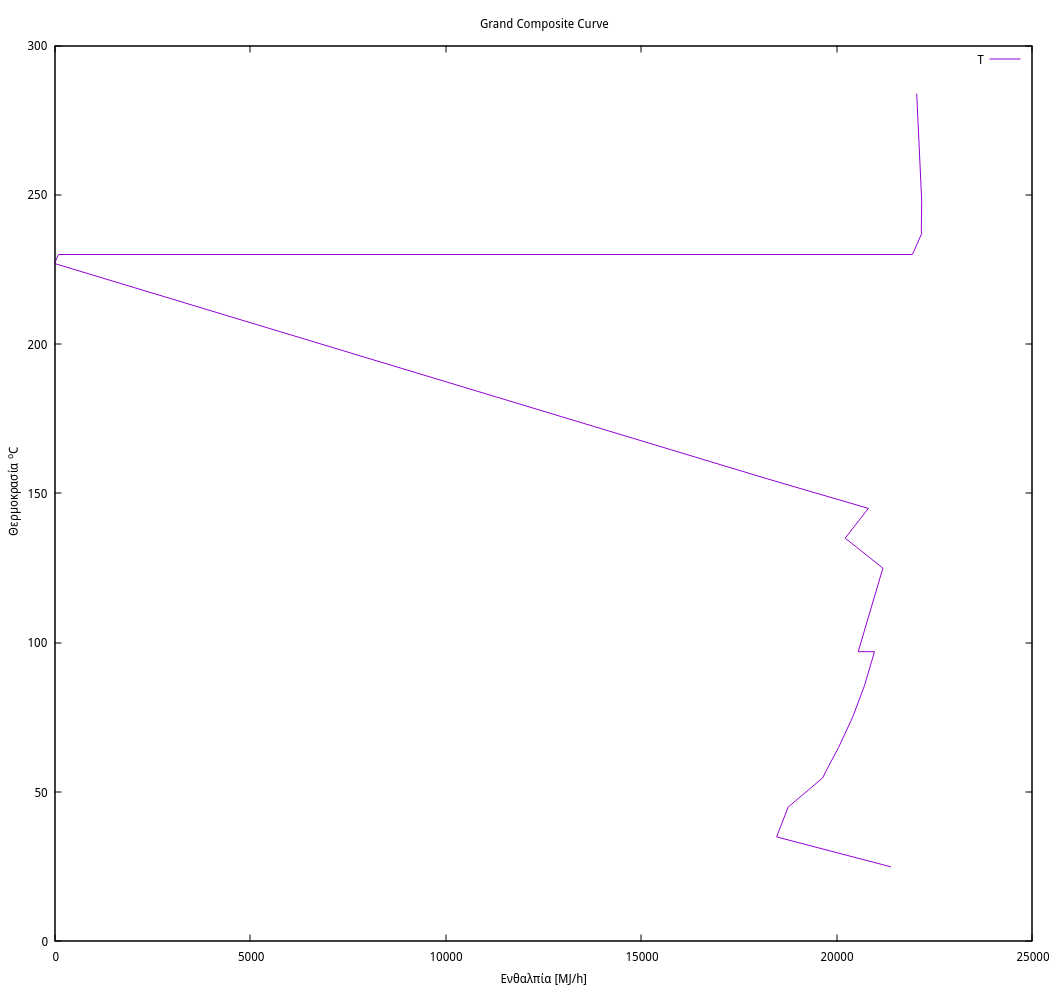
\includegraphics[width=.9\linewidth]{Diagrams/grand_composite_curve.png}
\caption{Μεγάλο Σύνθετο Γράφημα}
\end{figure}

Παρατηρούμε πως ο κόμβος ανάσχεσης είναι στους 227 \(^oC\) το οποίο σημαίνει πως τα περισσότερα θερμά ρεύματα που υπάρχουν δεν μπορούν να συνεισφέρουν στην λανθάνουσα θερμότητα του ατμού που τροφοδοτείται για την έκρηξη ατμού. Επίσης φαίνεται πως μία μεγάλη ενθαλπία απαιτείται για ψύξη, η οποία εν μέρει ευθύνεται και αυτή στην λανθάνουσα θερμότητα υδατικών ρευμάτων. Σε πρώτη φάση θα δούμε τι μπορεί να ολοκληρωθεί στην διεργασία.

\subsection{Σχόλια για την ολοκλήρωση διάφορων κομματιών}
\label{sec:org24824f7}
\subsubsection{Αντιδραστήρας παραγωγής γλυκερόλης}
\label{sec:orgc9c83c1}
Ο αντιδραστήρας λειτουργεί στους 30 βαθμούς κελσίου και είναι εξώθερμος. Στο μεγάλο σύνθετο γράφημα θα έμπαινε στους 25 \(^oC\) το οποίο είναι κάτω από τον κόμβο ανάσχεσης. Λόγω της πολύ στενής θερμοκρασιακής περιοχής στην οποία μπορεί να διεξαχθεί η αντίδραση, θεωρούμε πως δεν αξίζει να μελετηθεί ένα σενάριο ολοκλήρωσης του αντιδραστήρα αυτού με την υπόλοιπη διεργασία, καθώς σε κάθε περίπτωση απλώς θα αυξάνει την απαίτηση σε ψυχρή παροχή.
\subsubsection{Αποστακτική στήλη γλυκερόλης}
\label{sec:org3900447}
Ο αναβραστήρας της στήλης λειτουργεί στους 293 \(^oC\) στο ΜΣΓ και έχει απαίτηση θερμότητας στους 1105.44 MJ/hr. O συμπηκνωτήρας της στήλης λειτουργεί στους 145 \(^oC\) (140 \(^oC\) στο ΜΣΓ) με απαίτηση 149.46 MJ/hr. Καθώς ο κόμβος ανάσχεσης είναι στους 227 \(^oC\) και το 293 \(^oC\) υπερβαίνει τις θερμοκρασίες που εμφανίζονται στο ΜΣΓ για να ολοκληρωθεί η στήλη θα έπρεπε σε πρώτη φάση να λειτουργεί σε συνθήκες μειωμένης πίεσης (πχ απόσταξη υπό κενό). Λόγω του αρκετά αυξημένου λειτουργικού κόστους μίας τέτοιας διεργασίας, κρίνεται ακατάλληλο ως ιδέα.
\subsubsection{Αντιδραστήρας παραγωγής φουρφουράλης}
\label{sec:org3013e5c}
Θερμοκρασία λειτουργίας οι 242 \(^oC\), ή 237 \(^oC\) στο μεγάλο σύνθετο γράφημα. Ο αντιδραστήρας είναι εξώθερμος, και λειτουργεί ισοθερμοκρασιακά πάνω από τον κόμβο ανάσχεσης. Επίσης, η απαίτηση του σε ψύξη είναι αρκετά χαμηλή (13.35 MJ/hr) άρα είναι αρκετά εύκολο να χωρέσει. Η ολοκλήρωση του βελτιώνει την διεργασία, βέβαια λόγω του πολύ μικρού θερμικού φορτίου, την βελτιώνει ελάχιστα.
\subsubsection{Αντιδραστήρας παραγωγής κυκλοπεντανόνης}
\label{sec:orgb106811}
Ο αντιδραστήρας αυτός λειτουργεί στους 160 \(^oC\) και είναι εξώθερμος (ως αντίδραση υδρογόνωσης). Αυτό είναι κάτω από τον κόμβο ανάσχεσης και μάλιστα αρκετά, άρα η ολοκλήρωση δεν θεωρείται εφικτή.
\subsubsection{Αποστακτική στήλη κυκλοπεντανόνης}
\label{sec:org4481ac8}
Ο συμπηκνωτήρας είναι ένα θερμό ρεύμα στους 50 \(^oC\) (45 \(^oC\) στο ΜΣΓ) με θερμότητα 8971.67 MJ/hr ενώ ο αναβραστήρας είναι ένα ψυχρό ρεύμα στους 130 (135 \(^oC\) στο ΜΣΓ) με θερμότητα 9545.79 MJ/hr. Και οι 2 θερμοκρασίες είναι κάτω από τον κόμβο ανάσχεσης και υπάρχει σίγουρα το περιθώριο να γίνει μία ολοκλήρωση. Η ολοκλήρωση της στήλης θα γίνει αφαιρώντας 9545.79 MJ/hr στη θερμοκρασία του αναβραστήρα και επιστρέφοντας 8971.67 MJ/hr στην θερμοκρασία του συμπηκνωτήρα.
\subsubsection{Αντιδραστήρας σακχαροποίησης}
\label{sec:org2eae97c}
Ο αντιδραστήρας λειτουργεί στους 50 \(^oC\) και είναι ενδόθερμος (45 στο ΜΣΓ). Είναι κάτω από τον κόμβο ανάσχεσης και έχει απαίτηση 393.63 MJ/hr άρα η ολοκλήρωση του είναι αρκετά εύκολη.

\subsubsection{Αλλαγές στο ΜΣΓ}
\label{sec:org0f6e26f}
Η ολοκλήρωση των αντιδραστήρων παραγωγής της φουρφουράλης και της σακχαροποίησης είναι εφικτή και μειώνει την απαίτηση της διεργασίας σε θερμά και ψυχρά ρεύματα αντίστοιχα, παρόλο που η επίδραση τους δεν είναι τόσο μεγάλη. Η αποστακτική της φουρφουράλης προκαλεί μία σημαντική αλλαγή στο ΜΣΓ η οποία οδηγεί στον διαχωρισμό να είναι πρακτικά δωρεάν και να δημιουργείται και μία ενεργειακή τσέπη λόγω της ολοκλήρωσης αυτής.

Παρακάτω παρατίθεται και το ΜΣΓ στο οποίο έχουν γίνει οι δύο αυτές προσθήκες.
\begin{table}[htbp]
\caption{Δεδομένα για τον ενεργειακό καταρράκτη}
\centering
\begin{tabular}{rr}
Cumulative  Dh & T\\
\hline
22029.075 & 283.9\\
22157.741 & 248\\
22146.601 & 238\\
22169.010 & 237\\
21931.525 & 230.01\\
101.925 & 230\\
0 & 227\\
18195 & 155\\
20806.8 & 145\\
20473.65 & 139.4\\
20215.16 & 135\\
10669.37 & 135\\
11632.97 & 125\\
11000.68 & 97.01\\
11418.51 & 97\\
11162.11 & 85.65\\
10875.63 & 75.65\\
10852.067 & 74.9\\
10495.957 & 64.9\\
10174.817 & 56.97\\
10093.383 & 54.75\\
9210.243 & 45\\
18181.913 & 45\\
18066.363 & 35\\
20977 & 25\\
\end{tabular}
\end{table}

\begin{figure}[htbp]
\centering
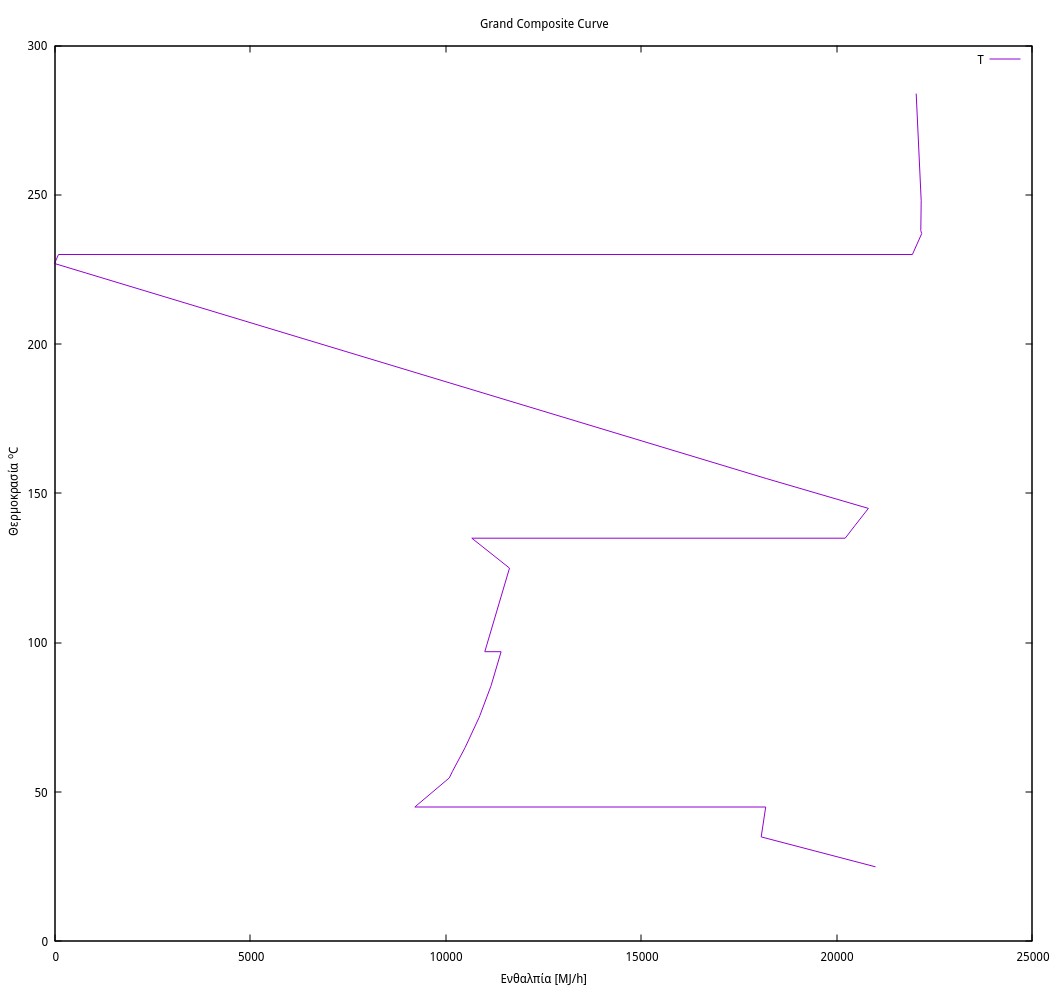
\includegraphics[width=.9\linewidth]{Diagrams/grand_composite_curve_2.png}
\caption{Μεγάλο Σύνθετο Γράφημα μετά την ολοκλήρωση 3 διεργασιών}
\end{figure}

\subsection{Περαιτέρω εκμετάλλευση της περιοχής κάτω από τον κόμβο ανάσχεσης}
\label{sec:org228dd4d}
Ακόμη και μετά την ολοκλήρωση των διεργασιών αυτών βλέπουμε πως υπάρχει μία μεγάλη αυτόνομη περιοχή από τουυς 45 \(^oC\) μέχρι τους 190 \(^oC\). Βλέποντας έτσι το ΜΣΓ, 11766.8 MJ/hr ψυχρή παροχή απαιτείται για ψύξη ρευμάτων σε θερμοκρασίες από 45 \(^oC\) και κάτω. Τα υπόλοιπα 9210.2 MJ/hr χρησιμοποιούνται για ψύξη ρευμάτων σε θερμοκρασίες από 190 \(^oC\) εώς 227 \(^oC\). Το βασικό θερμό ρεύμα στην περιοχή αυτή είναι οι ατμοί της έκρηξης ατμού μετά την διεργασία εκείνη. Είναι ατμός σε πολύ υψηλή πίεση (26 bar) ο οποίος μπορεί να χρησιμοποιηθεί για την ολοκλήρωση διάφορων κομματιών και παραμένει ένα αρκετά θερμό ρεύμα για ατμοπαραγωγή.

Η θερμοκρασία 190 \(^oC\) για ένα θερμό είναι στην πραγματικότητα 185 \(^oC\). Άρα, η παραγωγή ατμού μπορεί να γίνει στους 175 \(^oC\) μέγιστο. Η πίεση στην οποία το νερό αυτό θα υγροποιούνταν είναι 8.93 bar, άρα για ατμοπαραγωγή η υψηλότερη βαθμίδα πίεσης που μπορούμε να χρησιμοποιήσουμε είναι τα 8.5 bar.  Με βάση το θερμικό περιεχόμενο που υπάρχει διαθέσιμο, μπορεί η παροχή του ατμού αυτού να είναι 176.7 kmol/hr. Άρα, για να μειώσουμε τις απαιτήσεις σε ψυχρή παροχή, βάζουμε ένα νέο ψυχρό ρεύμα στο ΜΣΓ το οποίο πάει από τους 25 \(^oC\) στους 180 \(^oC\). Η αισθητή θερμότητα της μεταβολής είναι 2389.9 MJ/hr μέχρι τους 178.1 \(^oC\), η λανθάνουσα (θα βάλουμε στον πίνακα μεταβολή από 178.1 μέχρι 178.2) θα έχει μεταβολή 6804.2 MJ/hr και τα υπόλοιπα 16 είναι από τους 178.2 μέχρι τους 180.

\begin{table}[htbp]
\caption{Δεδομένα για τον ενεργειακό καταρράκτη με ατμοπαραγωγή}
\centering
\begin{tabular}{rr}
Cumulative  Dh & T\\
\hline
22029.075 & 283.9\\
22157.741 & 248\\
22146.601 & 238\\
22169.010 & 237\\
21931.525 & 230.01\\
101.924 & 230\\
0 & 227\\
12220 & 178.2\\
5415.8 & 178.2\\
11033.056 & 155\\
13490.656 & 145\\
13071.154 & 139.4\\
12744.816 & 135\\
3199.029 & 135\\
4008.425 & 125\\
2944.530 & 97.01\\
3362.205 & 97\\
2930.789 & 85.65\\
2490.108 & 75.65\\
2454.980 & 74.9\\
1944.670 & 64.9\\
1501.250 & 56.97\\
1385.583 & 54.75\\
352.099 & 45\\
9323.769 & 45\\
9054.019 & 35\\
11810.456 & 25\\
\end{tabular}
\end{table}

\begin{figure}[htbp]
\centering
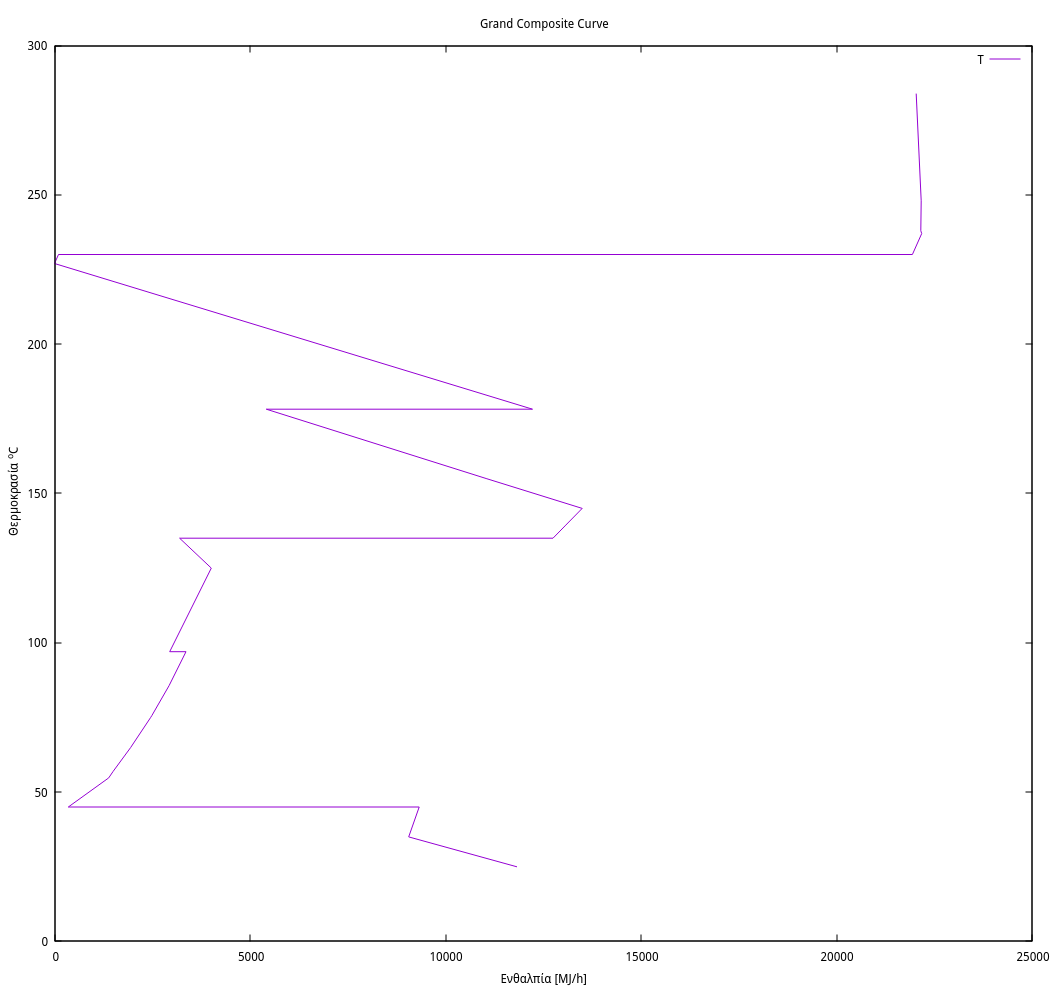
\includegraphics[width=.9\linewidth]{Diagrams/grand_composite_curve_3.png}
\caption{Μεγάλο Σύνθετο Γράφημα μετά την ενσωμάτωση ατμοπαραγωγής}
\end{figure}

Έτσι, μειώνουμε σημαντικά την απαίτηση σε ψυχρές παροχές καθώς πλέον μόνο ότι χρειάζεται κάτω από τους 45 \(^oC\) πρέπει να δωθεί από ψυχρές παροχές και η υπόλοιπη απαίτηση δεν θεωρείται ψυχρή παροχή, αλλά ενσωματωμένη ατμοπαραγωγή. Ότι είναι πάνω από την περιοχή αυτή έχει γίνει πρακτικά αυτόνομη περιοχή λόγω της μεγάλης τσέπης που έχει δημιουργηθεί.

\subsection{Συμπεράσματα της ενεργειακής ολοκλήρωσης}
\label{sec:orgdd5426c}
Συμπέρασμα ότι με την ενεργειακή ολοκλήρωση αυτή έχουμε τα εξής:

Απαίτηση σε ψυχρή παροχή 11810.46 MJ/h σε θερμοκρασία κάτω από 25 \(^oC\) στο ΜΣΓ (δηλαδή κάτω από 20 \(^oC\), άρα στους 15 \(^oC\) πχ).

Απαίτηση σε θερμή παροχή: 22029.08 MJ/h. Αυτό πρακτικά οφείλεται στην λανθάνουσα θερμότητα του ατμού που χρησιμοποιείται στο steam explosion και θα καλυφθεί εκμαστεύοντας μία ποσότητα ατμού σε υψηλή πίεση (60 bar) από το ενσωματωμένο κύκλο Rankine της διεργασίας με παροχή τέτοια ώστε να επαρκεί για να καλύψει την ανάγκη αυτή. Ο ατμός αυτός βγαίνει στους 497.5 \(^oC\) από τον στρόβιλο υψηλής πίεσης και θα αξιοποιηθεί ως έχει καθώς η παροχή του είναι ρυθμισμένη για να καλύψει την απαίτηση που υπάρχει. Μετά την εναλλαγή, ανακυκλώνεται στο κύκλο Rankine μιας και δεν μπορεί να γίνει κάτι άλλο.

Επίσης πρέπει να υπάρχουν διαθέσιμες ψυχρές παροχές για την ψύξη των αντιδραστήρων παραγωγής φουρφουράλης και γλυκερόλης, του συμπηκνωτήρα της αποστακτικής στήλης της γλυκερόλης και τέλος θερμή παροχή για τον αναβραστήρα της στήλης εκείνης.

\section{Σχεδιασμός δικτύου εναλλαγής θερμότητας}
\label{sec:org820da2a}
Έχοντας δει όλη την διεργασία και έχοντας κάνει την βέλτιστη δυνατή ενεργειακή ολοκλήρωση, πρέπει να σχεδιαστεί ένα δίκτυο εναλλαγής θερμότητας για την διεργασία με βάση το οποίο θα βρούμε ποιό ρεύμα εναλλάσει με ποιό. Αρχικά, αξίζει να δούμε σε έναν πίνακα όλα τα ρεύματα της διεργασίας και ότι θέλουμε να ολοκληρώσουμε.

\begin{table}[htbp]
\caption{Ρεύματα της διεργασίας}
\centering
\begin{tabular}{llrrr}
Ρεύμα & Είδος & CP (MJ/h K) & Τ\textsubscript{in} (C) & T\textsubscript{out} (C)\\
\hline
FeedSteam & Ψυχρό & 47.732 & 25 & 237\\
StExpVapors & Θερμό & 65.487 & 227 & 25\\
CellLig & Θερμό & 7.654 & 227 & 75.65\\
NaOH & Ψυχρό & 6.058 & 25 & 85.65\\
Bleach & Ψυχρό & 4.192 & 25 & 74.9\\
Cellulose & Θερμό & 4.884 & 75.65 & 64.9\\
PureCell & Θερμό & 3.813 & 56.97 & 44.75\\
SachWater & Ψυχρό & 53.897 & 25 & 54.75\\
Glucose & Θερμό & 53.468 & 45 & 25\\
RProd & Ψυχρό & 57.746 & 35 & 145\\
FlashVapors & Θερμό & 53.681 & 135 & 25\\
GlycWater & Θερμό & 0.740 & 139.4 & 25\\
PureGlyc & Θερμό & 3.583 & 283.9 & 25\\
XylFeed & Ψυχρό & 4.698 & 237 & 248\\
FurFeed & Θερμό & 10.173 & 238 & 155\\
CyclProd & Θερμό & 15.066 & 155 & 25\\
Cycl & Θερμό & 4.676 & 125 & 25\\
Tol & Θερμό & 8.32 & 45 & 25\\
FurfReac & Θερμό & 7.436 & 237 & 237\\
SachReac & Ψυχρό & 55.589 & 45 & 45\\
CyclCond & Θερμό & 8.32 & 45 & 45\\
CyclBoil & Ψυχρό & 4.676 & 135 & 135\\
IntSteam & Ψυχρό & 13.32 & 25 & 180\\
\end{tabular}
\end{table}

Για τον υπολογισμό της θερμοχωρητικότητας των ρευμάτων των 2 αντιδραστήρων, καθώς μεταβάλλεται, προσεγγίζουμε την τιμή της ως τον μέσο όρο του ρεύματος εισόδου και του ρεύματος εξόδου. Για την αποστακτική, το CP είναι ίδιο με το CP του αντίστοιχου προιόντος καθώς δεν υπάρχει χημική μεταβολή στον συμπηκνωτήρα ή τον αναβραστήρα. Τέλος, για το ρεύμα IntSteam (ενσωματωμένη ατμοπαραγωγή), ξέρουμε την παροχή που μπορούμε να προσφέρουμε στο σύστημα με βάση το ΜΣΓ και άρα υπολογίζεται εύκολα το CP.

Με βάση τις πληροφορίες αυτές μπορεί να φτιαχτεί το διάγραμμα πλέγματος της διεργασίας πάνω στο οποίο θα βασιστεί και ο σχεδιασμός του δικτύου εναλλαγής θερμότητας. Αξίζει να αναφερθεί πως στο διάγραμμα πλέγματος που παρατίθεται φαίνονται και οι εναλλάκτες που θα χρησιμοποιηθούν. Η διαδικασία με την οποία τοποθετήθηκαν φαίνεται παρακάτω.

\begin{figure}[htbp]
\centering
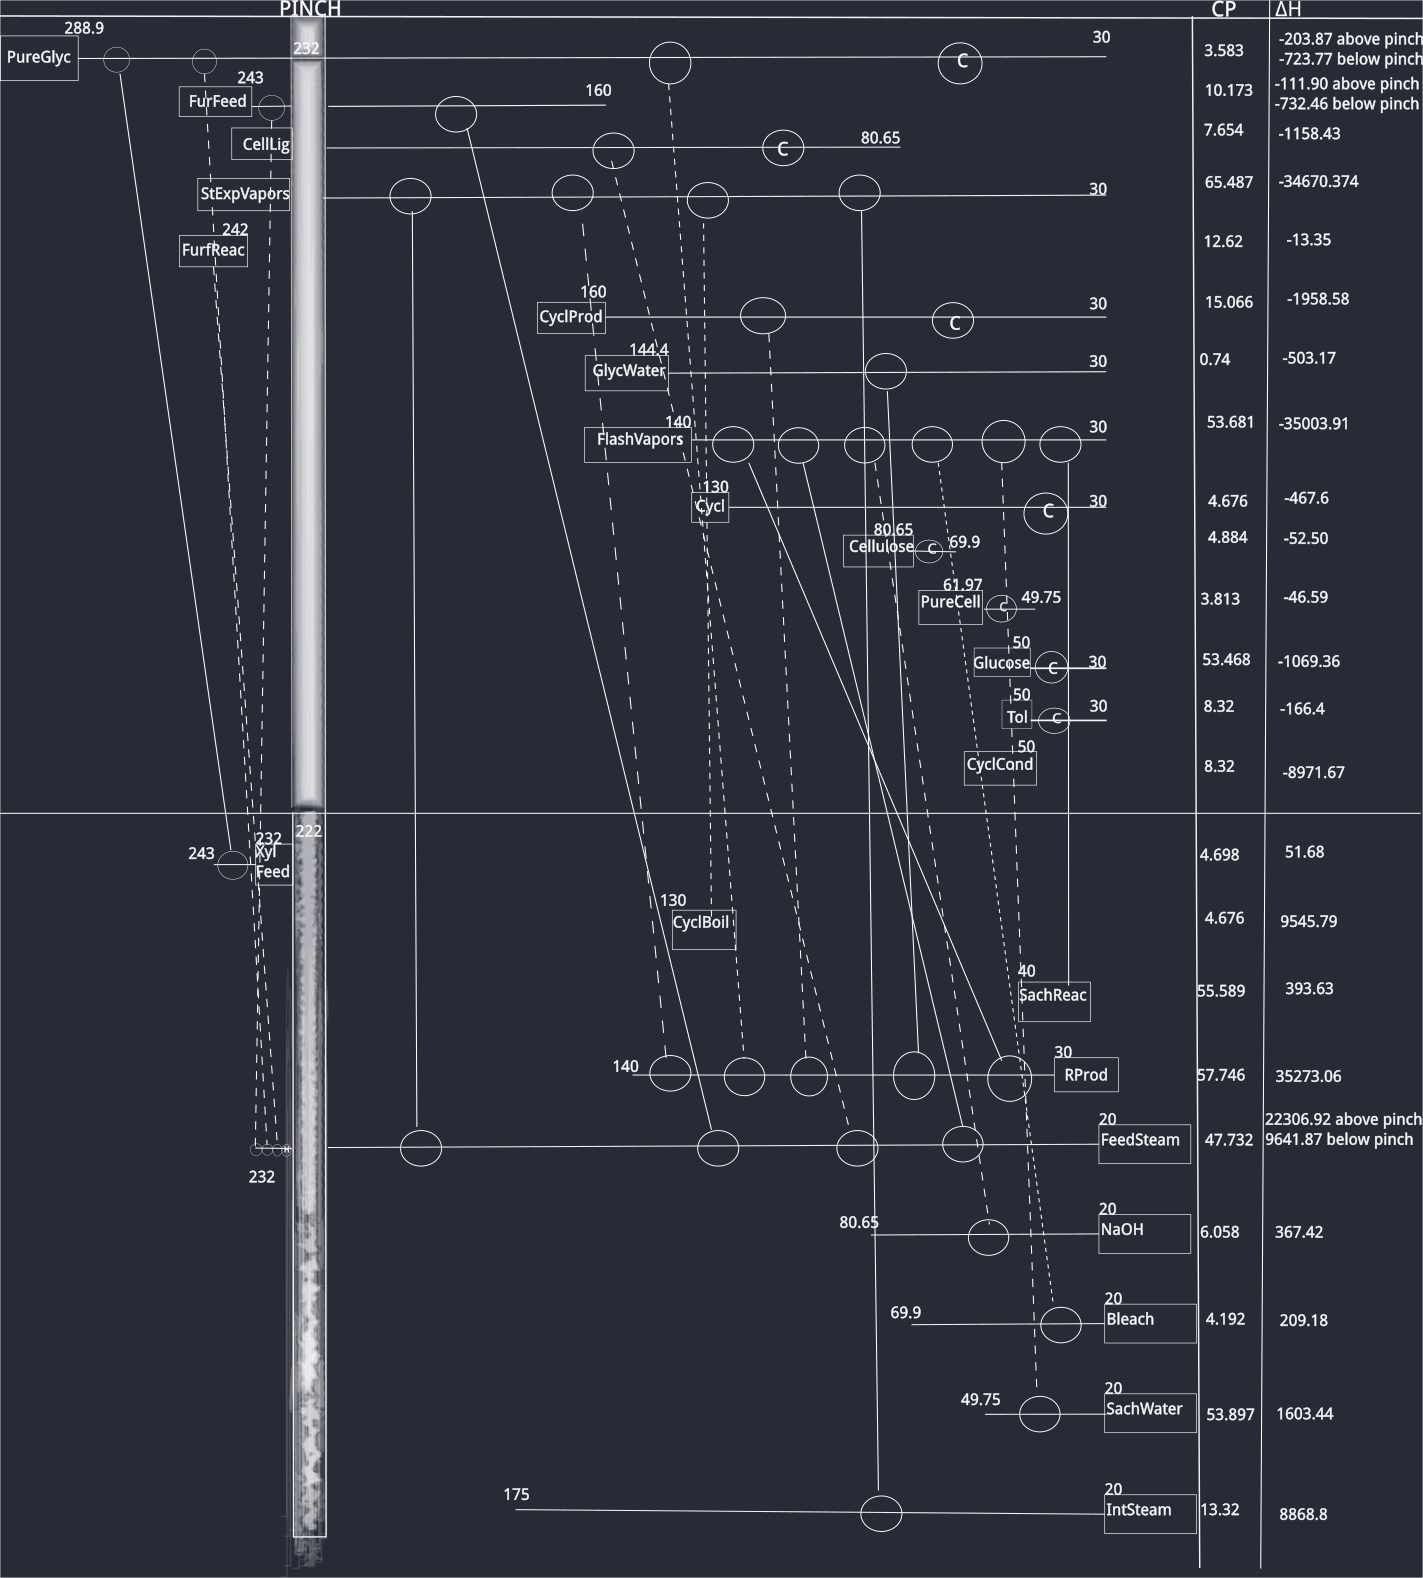
\includegraphics[width=.9\linewidth]{Diagrams/grid_diagram.png}
\caption{Διάγραμμα Πλέγματος της διεργασίας}
\end{figure}

Από το διάγραμμα πλέγματος, είναι εμφανές πως το κομμάτι της διεργασίας που βρίσκεται πάνω από τον κόμβο ανάσχεσης είναι αρκετά απλό (3 θερμά και 2 ψυχρά) ενώ το κομμάτι κάτω από τον κόμβο ανάσχεσης θέλει αρκετή δουλειά. Η λύση που προτείνεται για την περιοχή πάνω από τον κόμβο είναι μάλλον μία από τις καλύτερες δυνατές καθώς δεν υπάρχουν πολλοί βαθμοί ελευθερίας λόγω των λίγων ρευμάτων. Και έτσι και αλλιώς και χωρίς να γινόταν καθόλου ολοκλήρωση, η ουσιαστική απαίτηση που υπάρχει σε αυτό το θερμοκρασιακό εύρος είναι η θέρμανση του FeedSteam.

Αντίθετως κάτω από τον κόμβο ανάσχεσης, υπάρχουν πάρα πολλά ρεύματα και πρακτικά άπειροι δυνατοί συνδυασμοί καθώς μόνο ένα ρεύμα έχει υποχρεωτικό βαθμό ελευθερίας επειδή μπαίνει στον κόμβο ανάσχεσης. Ως αποτέλεσμα, το δίκτυο εναλλαγής που θα προταθεί δεν θα είναι σίγουρα το καλύτερο δυνατό αλλά μόνο ένα πιθανό σενάριο το οποίο δεν έχει πάρα πολύ μεγάλη απόκλιση από το βέλτιστο. Για να βρεθεί το πραγματικό βέλτιστο θα απαιτούνταν μία βελτιστοποίηση σε κατάλληλο λογισμικό (όπως πχ το GAMS). Όμως, ακόμη και εκεί, το πρόβλημα βελτιστοποίησης θα ήταν πάρα πολύ περίπλοκο λόγω του πλήθους των ρευμάτων. Σίγουρα ούτε ο αλγόριθμος βελτιστοποίησης θα έβρισκε την πραγματικά βέλτιστη λύση, αλλά ένα τοπικό ακρότατο, το οποίο ενδέχεται να ήταν και μία πολύ περίπλοκη και όχι πρακτικά εφικτή λύση. Για αυτό, δεν έγινε κάποια προσπάθεια να φτάσουμε έστω και κοντά στο πραγματικό βέλτιστο και απλώς αποδεχτήκαμε την απλούστερη δυνατή δομή του δικτύου η οποία ολοκληρώνει τα ρεύματα που είναι σημαντικό να ολοκληρωθούν μεταξύ τους.

\subsection{Υπολογισμός Ενθαλπιών}
\label{sec:orgb65cd67}
Για να μπορέσουμε να κάνουμε τους υπολογισμούς του δικτύου, πρέπει πρώτα να φτιάξουμε έναν συγκεντρωτικό πίνακα που δείχνει την ενθαλπία κάθε ρεύματος ξεχωριστά.

\begin{table}[htbp]
\caption{Συγκεντρωτικός πίνακας ρευμάτων με ενθαλπίες}
\centering
\begin{tabular}{llrr}
Ρεύμα & Είδος & CP (MJ/h K) & ΔΗ\textsubscript{tot} (MJ/h)\\
\hline
PureGlyc & Θερμό & 3.583 & -927.6387\\
FurFeed & Θερμό & 10.173 & -844.359\\
CellLig & Θερμό & 7.654 & -1158.4329\\
StExpVapors & Θερμό & 65.487 & -34670.374\\
FurfReac & Θερμό & 7.436 & -13.35\\
CyclProd & Θερμό & 15.066 & -1958.58\\
GlycWater & Θερμό & 0.740 & -503.166\\
FlashVapors & Θερμό & 53.681 & -35003.91\\
Cycl & Θερμό & 4.676 & -467.6\\
Cellulose & Θερμό & 4.884 & -52.503\\
PureCell & Θερμό & 3.813 & -46.59486\\
Glucose & Θερμό & 53.468 & -1069.36\\
Tol & Θερμό & 8.32 & -166.4\\
CyclCond & Θερμό & 8.32 & -8971.67\\
\hline
XylFeed & Ψυχρό & 4.698 & 51.678\\
CyclBoil & Ψυχρό & 4.676 & 9545.79\\
SachReac & Ψυχρό & 55.589 & 393.63\\
RProd & Ψυχρό & 57.746 & 35273.06\\
FeedSteam & Ψυχρό & 47.732 & 31948.784\\
NaOH & Ψυχρό & 6.058 & 367.4177\\
Bleach & Ψυχρό & 4.192 & 209.1808\\
SachWater & Ψυχρό & 53.897 & 1603.4358\\
IntSteam & Ψυχρό & 13.32 & 8868.8\\
\end{tabular}
\end{table}

Από αυτά τα ρεύματα, 3 (PureGlyc, FurFeed, FeedSteam) παιρνούν μέσα από τον κόμβο ανάσχεσης, άρα η ενθαλπία αυτή δεν είναι χαρακτηριστική και πρέπει να χωρίσει στα 2. Για τα ρεύματα PureGlyc και FurFeed, η αλλαγή έγκειται απλώς σε δύο υπολογισμούς της λανθάνουσας θερμότητας αντί για έναν. Στο FeedSteam, όλη η λανθάνουσα είναι πάνω από τον κόμβο ανάσχεσης ενώ απαιτούνται 2 υπολογισμοί για την αισθητή. Στον παρακάτω πίνακα τα ρεύματα αυτά έχουν χωριστεί με χρήση δεικτών a (above pinch) και b (below pinch).

\begin{table}[htbp]
\caption{Συγκεντρωτικός πίνακας ρευμάτων με ενθαλπίες}
\centering
\begin{tabular}{llrr}
Ρεύμα & Είδος & CP (MJ/h K) & ΔΗ\textsubscript{tot} (MJ/h)\\
\hline
PureGlyc\textsubscript{a} & Θερμό & 3.583 & -203.8727\\
PureGlyc\textsubscript{b} & Θερμό & 3.583 & -723.766\\
FurFeed\textsubscript{a} & Θερμό & 10.173 & -111.903\\
FurFeed\textsubscript{b} & Θερμό & 10.173 & -732.456\\
CellLig & Θερμό & 7.654 & -1158.4329\\
StExpVapors & Θερμό & 65.487 & -34670.374\\
FurfReac & Θερμό & 7.436 & -13.35\\
CyclProd & Θερμό & 15.066 & -1958.58\\
GlycWater & Θερμό & 0.740 & -503.166\\
FlashVapors & Θερμό & 53.681 & -35003.91\\
Cycl & Θερμό & 4.676 & -467.6\\
Cellulose & Θερμό & 4.884 & -52.503\\
PureCell & Θερμό & 3.813 & -46.59486\\
Glucose & Θερμό & 53.468 & -1069.36\\
Tol & Θερμό & 8.32 & -166.4\\
CyclCond & Θερμό & 8.32 & -8971.67\\
\hline
XylFeed & Ψυχρό & 4.698 & 51.678\\
CyclBoil & Ψυχρό & 4.676 & 9545.79\\
SachReac & Ψυχρό & 55.589 & 393.63\\
RProd & Ψυχρό & 57.746 & 35273.06\\
FeedSteam\textsubscript{a} & Ψυχρό & 47.732 & 22306.92\\
FeedSteam\textsubscript{b} & Ψυχρό & 47.732 & 9641.864\\
NaOH & Ψυχρό & 6.058 & 367.4177\\
Bleach & Ψυχρό & 4.192 & 209.1808\\
SachWater & Ψυχρό & 53.897 & 1603.4358\\
IntSteam & Ψυχρό & 13.32 & 8868.8\\
\end{tabular}
\end{table}

\subsection{Δίκτυο εναλλαγής θερμότητας πάνω από τον κόμβο ανάσχεσης}
\label{sec:org20672d9}
Πάνω από τον κόμβο ανάσχεσης έχουμε τα εξής ρεύματα

\begin{table}[htbp]
\caption{Ρεύματα πάνω από τον κόμβο ανάσχεσης}
\centering
\begin{tabular}{llrr}
Ρεύμα & Είδος & CP (MJ/h K) & ΔΗ\textsubscript{tot} (MJ/h)\\
\hline
PureGlyc\textsubscript{a} & Θερμό & 3.583 & -203.8727\\
FurFeed\textsubscript{a} & Θερμό & 10.173 & -111.903\\
FurfReac & Θερμό & 7.436 & -13.35\\
\hline
XylFeed & Ψυχρό & 4.698 & 51.678\\
FeedSteam\textsubscript{a} & Ψυχρό & 47.732 & 22306.92\\
\end{tabular}
\end{table}

Ξεκινάμε από τον κόμβο ανάσχεσης. Θέλουμε τα ρεύματα που μπαίνουν στον κόμβο (θερμά) να είναι λιγότερα ή ίσα από αυτά που βγαίνουν (ψυχρά) και τα θερμά να έχουν μικρότερα CP από τα ψυχρά. Δεν ασχολούμαστε με το FurfReac (αντιδραστήρας παραγωγής φουρφουράλης) καθώς είναι μακριά από τον κόμβο. Άρα έχουμε 2 θερμά, 2 ψυχρά. Το ρεύμα PureGlyc έχει μικρότερο CP και από τα δύο ψυχρά άρα μπορεί να ταιριάξει με οποιοδήποτε ενώ το FurFeed έχει μεγαλύτερο CP από το XylFeed άρα πρέπει αναγκαστικά να ταιριάξει με το FeedSteam. Αν ταιριάξουμε άρα το PureGlyc με το XylFeed, το φορτίο που μπορούμε να χρησιμοποιήσουμε είναι 51.678 MJ/h το οποίο είναι όσο χρειάζεται το XylFeed. Το FurFeed, το υπόλοιπο PureGlyc και το FurfReac με αυτήν την σειρά μπορούν να εναλλάξουν με το FeedSteam καλύπτοντας όλες τους τις ενεργειακές απαιτήσεις, ενώ οι περίσσεια θερμότητας του FeedSteam θα καλυφθεί από θερμές παροχές.

\subsection{Δίκτυο εναλλαγής θερμότητας κάτω από τον κόμβο ανάσχεσης}
\label{sec:org61f92f4}
Κάτω από τον κόμβο ανάσχεσης έχουμε τα εξής ρεύματα.

\begin{table}[htbp]
\caption{Ρεύματα κάτω από τον κόμβο ανάσχεσης}
\centering
\begin{tabular}{llrr}
Ρεύμα & Είδος & CP (MJ/h K) & ΔΗ\textsubscript{tot} (MJ/h)\\
\hline
PureGlyc\textsubscript{b} & Θερμό & 3.583 & -723.766\\
FurFeed\textsubscript{b} & Θερμό & 10.173 & -732.456\\
CellLig & Θερμό & 7.654 & -1158.4329\\
StExpVapors & Θερμό & 65.487 & -34670.374\\
CyclProd & Θερμό & 15.066 & -1958.58\\
GlycWater & Θερμό & 0.740 & -503.166\\
FlashVapors & Θερμό & 53.681 & -35003.91\\
Cycl & Θερμό & 4.676 & -467.6\\
Cellulose & Θερμό & 4.884 & -52.503\\
PureCell & Θερμό & 3.813 & -46.59486\\
Glucose & Θερμό & 53.468 & -1069.36\\
Tol & Θερμό & 8.32 & -166.4\\
CyclCond & Θερμό & 8.32 & -8971.67\\
\hline
CyclBoil & Ψυχρό & 4.676 & 9545.79\\
SachReac & Ψυχρό & 55.589 & 393.63\\
RProd & Ψυχρό & 57.746 & 35273.06\\
FeedSteam\textsubscript{b} & Ψυχρό & 47.732 & 9641.864\\
NaOH & Ψυχρό & 6.058 & 367.4177\\
Bleach & Ψυχρό & 4.192 & 209.1808\\
SachWater & Ψυχρό & 53.897 & 1603.4358\\
IntSteam & Ψυχρό & 13.32 & 8868.8\\
\end{tabular}
\end{table}

Υπάρχουν 13 θερμά και 8 ψυχρά και αναμένεται να υπάρξει μία μεγάλη απάιτηση σε ψυχρή παροχή. Το σύστημα που θεωρήθηκε φαίνεται παρακάτω

\begin{center}
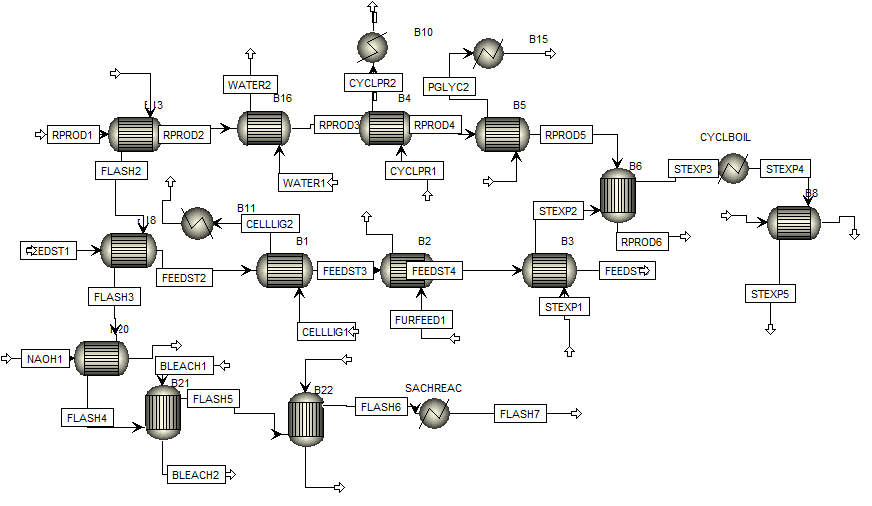
\includegraphics[width=.9\linewidth]{2023-04-14_19-38-26_screenshot.png}
\end{center}

\subsubsection{Επεξήγηση του συστήματος που θεωρήθηκε}
\label{sec:orgd8b8a49}
Βασιζόμαστε στο ότι τα δύο πιο απαιτητικά ψυχρά είναι το RProd και το FeedSteam. Και τα δύο προθερμαίνονται μέχρι τους 90 \(^oC\) με το FlashVapors το οποίο είναι το ρεύμα με τη μεγαλύτερη θερμοχωρητικότητα αλλά σε χαμηλή θερμοκρασία άρα δεν μπορεί να τα φτάσει μέχρι την τελική τους θερμοκρασία. Το ρεύμα αυτό μπορεί μετά την προθέρμανση αυτών να χρησιμοποιηθεί και γιά κάθε άλλο ψυχρό ρεύμα εκτός από τον αναβραστήρα της αποστακτικής της κυκλοπεντανόνης. Καταλήγει ως ένα μίγμα υγρού-ατμού χαμηλής ποιότητας.

Μετά την προθέρμανση, χρησιμοποιούμε όσα θερμά ρεύματα της διεργασίας έχουμε διαθέσιμα σε θερμοκρασίες πάνω από τους 90 \(^oC\) για να αυξήσουμε την θερμοκρασία των δύο ψυχρών και τα δύο ολοκληρώνονται από το StExpVapors, το άλλο σημαντικό θερμό ρεύμα της διεργασίας. Αυτό πρέπει πρώτα να εναλλάξει με το FeedSteam καθώς είναι το μόνο που μπορεί να το φέρει στους 222 \(^oC\) και άρα είναι υποχρεωτικός βαθμός ελευθερίας. Έπειτα θερμαίνει ότι χρειάζεται από το RProd, θερμαίνει τον αναβραστήρα της αποστακτικής της κυκλοπεντανόνης και τέλος, παράγει τον ενσωματωμένο ατμό της διεργασίας στα 8.5 bar. Μετά από όλα αυτά έχουμε εκμεταλλευτεί πρακτικά όλη την λανθάνουσα θερμότητα του ρεύματος, το οποίο καταλήγει ως ένα ρεύμα στους 166 \(^oC\) το οποίο όμως λόγω της υψηλής πίεσης είναι πλήρως υγροποιημένο (εκτός του αερίου CO\textsubscript{2} που έχει). Δεν έχει νόημα να το εκμεταλλευτούμε περαιτέρω καθώς δεν μπορεί να θερμάνει κάποιο άλλο ψυχρό και η χρήση του για ατμοπαραγωγή έχει πρακτικά εξαλειφθεί.

Τα ρεύματα Cellig, PureGlyc και CyclProd που έχουν χρησιμοποιηθεί σε ένα στάδιο της ολοκλήρωσης ψύχονται μέχρι τις θερμοκρασίες που πρέπει με ψυκτικό μέσο καθώς δεν βρέθηκε κάποιο ψυχρό ρεύμα για να εναλλάξει με αυτά μέχρι την τελική απαίτηση που υπήρχε, ενώ τα ρεύματα Cycl, Cellulose, PureCell, Glucose, Tol ψύχονται αποκλειστικά με ψυχρή παροχή. Βέβαια, οι απαιτήσεις όλων αυτών των ρευμάτων ανέρχονται περίπου στα 2500 MJ/hr. Αξίζει να σημειωθεί πως επίσης δεν έχει ολοκληρωθεί ο συμπηκνωτήρας της κυκλοπεντανόνης, ο οποίος έχει σημαντικό θερμικό φορτίο (περίπου 9000 MJ/hr). Αυτό βέβαια είναι σχετικά αναμενόμενο καθώς η περιοχή του ΜΣΓ η οποία χρειάζεται την ψυχρή παροχή έχει ένα μεγάλο οριζόντιο τμήμα που είναι αυτός ο συμπηκνωτήρας. Βέβαια, όπως είδαμε και πριν την ολοκλήρωση, η απαίτηση αυτή θα υπήρχε έτσι και αλλιώς, απλώς βάζοντας τον συμπηκνωτήρα πετυχαίνουμε καλύτερη ολοκλήρωση. Αν υποθέσουμε πως αφήνουμε τα πρακτικά υγρά υδατικά ρεύματα FlashVapors, StExpvapors και GlycWater στις θερμοκρασίες που είναι, η απαίτηση είναι 11500 MJ/h περίπου. Αν τα ψύξουμε μέχρι τους 20 \(^oC\) όπως θεωρήθηκε αρχικά για την δημιουργία του ΜΣΓ, είναι προφανές πως η απαίτηση σε ψυχρή παροχή θα είναι αρκετά μακριά από την θεωρητική ελάχιστη. Αυτό δείχνει κιόλας πως η επιλογή σίγουρα δεν είναι από τις καλύτερες. Όμως, η ψύξη των ρευμάτων αυτών, τα οποία έχουν ήδη εξαλείψει ένα αρκετά σημαντικό ποσόστο της θερμικής τους απαίτησης δεν είναι σίγουρο πως είναι απαραίτητη. Δεν υπάρχει κάποιο άλλο ρεύμα που αξίζει να προθερμάνουν και είναι πρακτικά στην υγρή φάση άρα σίγουρα δεν μπορούν να χρησιμοποιηθούν για ατμοπαραγωγή.

\section{Blocks της διεργασίας μετά την ενεργειακή ολοκλήρωση}
\label{sec:org349b1de}
Έχοντας δει την ενεργειακή ολοκλήρωση και το δίκτυο εναλλαγής θερμότητας που προτείνεται, έπρεπε να περαστεί αυτό και στα Aspen. Καθώς σε αρκετές περιπτώσεις έπρεπε να εναλλάξουν ρεύματα από διαφορετικά αρχεία Aspen (λόγω των πολλών blocks της διεργασίας), χρησιμοποιήθηκε μία πιο συστηματική ονοματολογία στα τελικά αρχεία ώστε να είναι εύκολο να δει κάποιος από ποιό σημείο της διεργασίας έρχεται ένα άλλο ρεύμα. Επίσης, η ονοματολογία βοηθάει και στην κοστολόγηση των εναλλακτών. Πολλοί εναλλάκτες μπαίνουν σε δύο αρχεία καθώς τα ρεύματα είναι από διαφορετικά αρχεία. Ο κανόνας που θα ακολουθηθεί είναι πως η κοστολόγηση τους θα γίνει στο block το οποίο αναφέρεται στο όνομα τους.

Η ονοματολογία θα βασιστεί σε ένα format A-XYY όπου το A θα είναι ένα γράμμα που παριστάνει τι διεργασία είναι κάτι, το X θα είναι ο αριθμός του block και τα YY θα είναι η αρίθμηση αυτών. Τα γράμματα Α θα είναι τα εξής

\begin{table}[htbp]
\caption{Ονοματολογία Διεργασίας}
\centering
\begin{tabular}{ll}
Γράμμα & Διεργασία\\
\hline
S & Ρεύμα Διεργασίας\\
HU & Θερμή Παροχή\\
CU & Ψυχρή Παροχή\\
R & Αντιδραστήρας\\
Τ & Στρόβιλος\\
P & Αντλία\\
D & Αποστακτική Στήλη\\
F & Απόσταξη Flash\\
Ε & Εκχύλιση\\
Η & Εναλλάκτης\\
M & Αναμίκτης\\
C & Φυγόκεντρος\\
O & Άλλα\\
\end{tabular}
\end{table}

Με την ονοματολογία να έχει καλυφθεί, παρακάτω παρατίθενται εικόνες από το Aspen για τα blocks όπου έχουν ενσωματωθεί όλοι οι εναλλάκτες της προτεινόμενης ενεργειακής ολοκλήρωσης. Αξίζει να σημειωθεί πως δεν θα συμπεριληφθούν φωτογραφίες για τα blocks 300 και 400 καθώς πρακτικά δεν συμμετέχουν στην ολοκλήρωση. Το 300 έχει μοναδική συνεισφορά την εναλλαγή με το FeedSteam το οποίο φαίνεται και στην προηγούμενη εικόνα ενώ το block 400 του βιοαντιδραστήρα δεν έχει μεταβολές στην θερμοκρασία.

\begin{figure}[htbp]
\centering
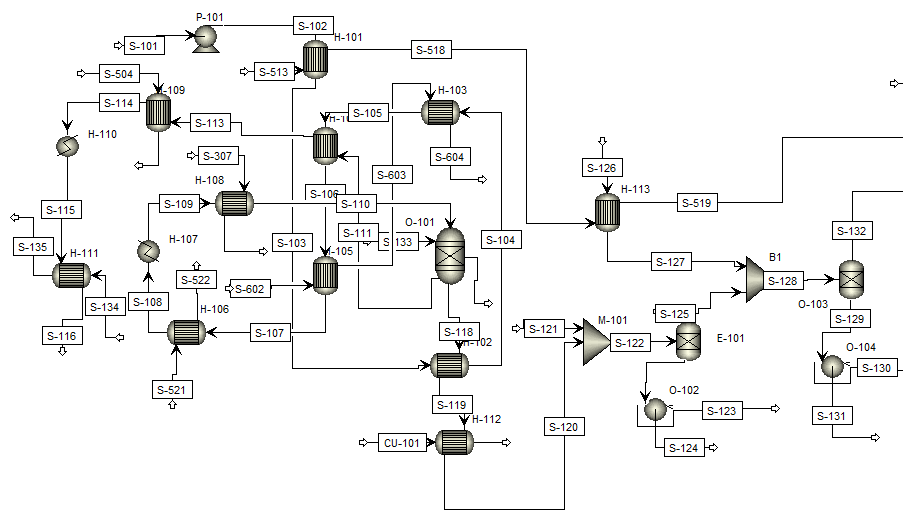
\includegraphics[width=.9\linewidth]{Blocks_της_διεργασίας_μετά_την_ενεργειακή_ολοκλήρωση/2023-04-27_14-47-13_screenshot.png}
\caption{Block 100 στο Aspen}
\end{figure}

Στο block 100 υπάρχουν το FeedSteam καθώς και το StExpvapors, δύο πολύ σημαντικά ρεύματα που συνεισφέρουν σε πολύ μεγάλο ποσοστό στο τελικό ΔΕΘ. Για αυτό, το αριστερά κομμάτι του block είναι πρακτικά ένα μεγάλο κομμάτι του δικτύου το οποίο βασίζεται στα δύο αυτά ρεύματα.

\begin{figure}[htbp]
\centering
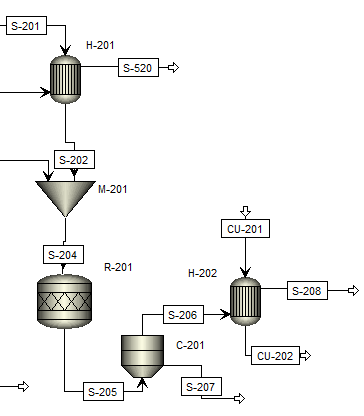
\includegraphics[height=250px]{Blocks_της_διεργασίας_μετά_την_ενεργειακή_ολοκλήρωση/2023-04-27_14-50-58_screenshot.png}
\caption{Block 200 στο Aspen}
\end{figure}


\begin{figure}[htbp]
\centering
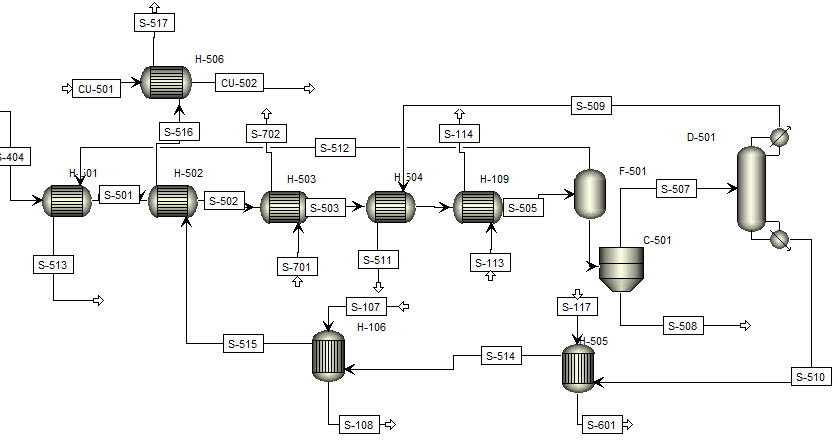
\includegraphics[width=.9\linewidth]{Blocks_της_διεργασίας_μετά_την_ενεργειακή_ολοκλήρωση/2023-04-27_14-54-20_screenshot.png}
\caption{Block 500 στο Aspen}
\end{figure}

Το block 500 είναι το άλλο αρχείο όπου υπάρχουν πάρα πολλοί εναλλάκτες όπως και στο 100, επειδή εδώ βρίσκονται τα άλλα 2 πολύ σημαντικά ρεύματα της διεργασίας, το RProd και το FlashVapors. Αξίζει να αναφερθεί πως χάριν ευκολίας δεν έχουν παρατεθεί οι εναλλαγές του FlashVapors πέρα από την 1η με το RProd καθώς όλες είναι πρακτικά στα block 100 και 200 όπου φαίνεται ότι μπαίνει το ρεύμα S-513 και κάνει όλες τις απαιτούμενες εναλλαγές.

\begin{figure}[htbp]
\centering
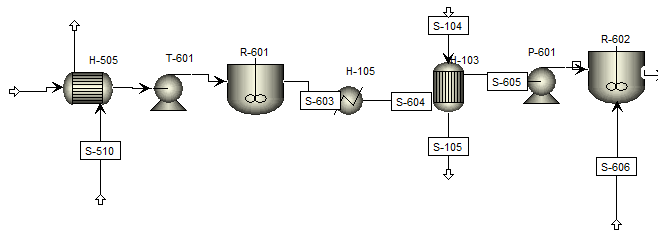
\includegraphics[width=.9\linewidth]{Blocks_της_διεργασίας_μετά_την_ενεργειακή_ολοκλήρωση/2023-04-27_15-00-23_screenshot.png}
\caption{Block 600 στο Aspen}
\end{figure}

Το block 600 έχει 3 εναλλάκτες οι οποίοι όμως έχουν ήδη συμπεριληφθεί και σε προηγούμενα αρχεία. Βέβαια, για κάποιον λόγο, η προσθήκη του H-105 ως HeatX είναι αδύνατη καθώς βγαίνει error. Ο εναλλάκτης σίγουρα λειτουργεί (και μπορεί κανείς να το δεί αυτό στο block 100) αλλά εδώ βγάζει error για αυτό προστέθηκε ως απλός heater.

\begin{figure}[htbp]
\centering
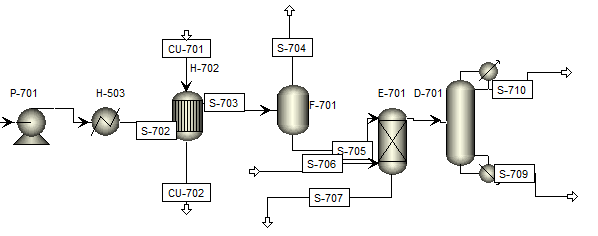
\includegraphics[width=.9\linewidth]{Blocks_της_διεργασίας_μετά_την_ενεργειακή_ολοκλήρωση/2023-04-27_15-02-15_screenshot.png}
\caption{Block 700 στο Aspen}
\end{figure}

\pagebreak

\section{Κοστολόγηση της διεργασίας}
\label{sec:orgae252f7}
Εφόσον έχει γίνει η ολοκλήρωση της διεργασίας, έχουμε πλέον την βέλτιστη δυνατή μονάδα και πρέπει να γίνει η ολοκληρωμένη κοστολόγηση της για να δούμε αν αξίζει ή όχι η επένδυση. Ξεκινάμε υπενθυμίζοντας το οικονομικό δυναμικό της διεργασίας, το οποίο είχε προκύψει ίσο με 98.2 εκατομμύρια ευρώ το έτος. Αυτό το νούμερο αποτελεί το όριο του κόστους που θεωρείται αποδεκτό.

Στην ολοκληρωμένη κοστολόγηση υπάρχει ένα επιπλέον προιόν της διεργασίας, το οποίο είναι η ηλεκτρική ενέργεια που παράγεται από την λιγνίνη και είναι πάρα πολύ σημαντική σε ποσότητα. Επίσης, υπάρχει και το κόστος των βοηθητικών παροχών. Όμως, πρακτικά μόνο οι ψυχρές είναι που θα κοστολογηθούν καθώς το κύκλο συμπαραγωγής παράγει όση θερμή παροχή και όση ηλεκτρική ενέργεια χρειάζεται.

Επίσης, η ολοκληρωμένη κοστολόγηση θα περιλαμβάνει προφανώς και τον εξοπλισμό όλων των διεργασιών, το οποίο θεωρείται πως θα είναι το μεγαλύτερο κόστος της διεργασίας.
\end{document}